\chapter{Experiment}
\begin{chapterabstract}
This chapter will describe the~production of the~experiment scene. It deals with the~transfer of the~original model to the~Unreal Engine project and finally with the~deployment of the~plug-in produced in Chapter~\ref{chap:implementation}.
\end{chapterabstract}

\section{Scene}
The~scene was made in Blender~\cite{blender} and transferred to an~Unreal project, which can be found in the~enclosed media in the~\path{experiment/project/CNB_NC_ET.zip} file. Opening this unreal project may require compilation. All later introduced Blueprints are found in this project. The~entire level in the~Unreal project can be seen in Figure~\ref{fig:unreal-cnb-level}.

\begin{figure}[!ht]\centering
    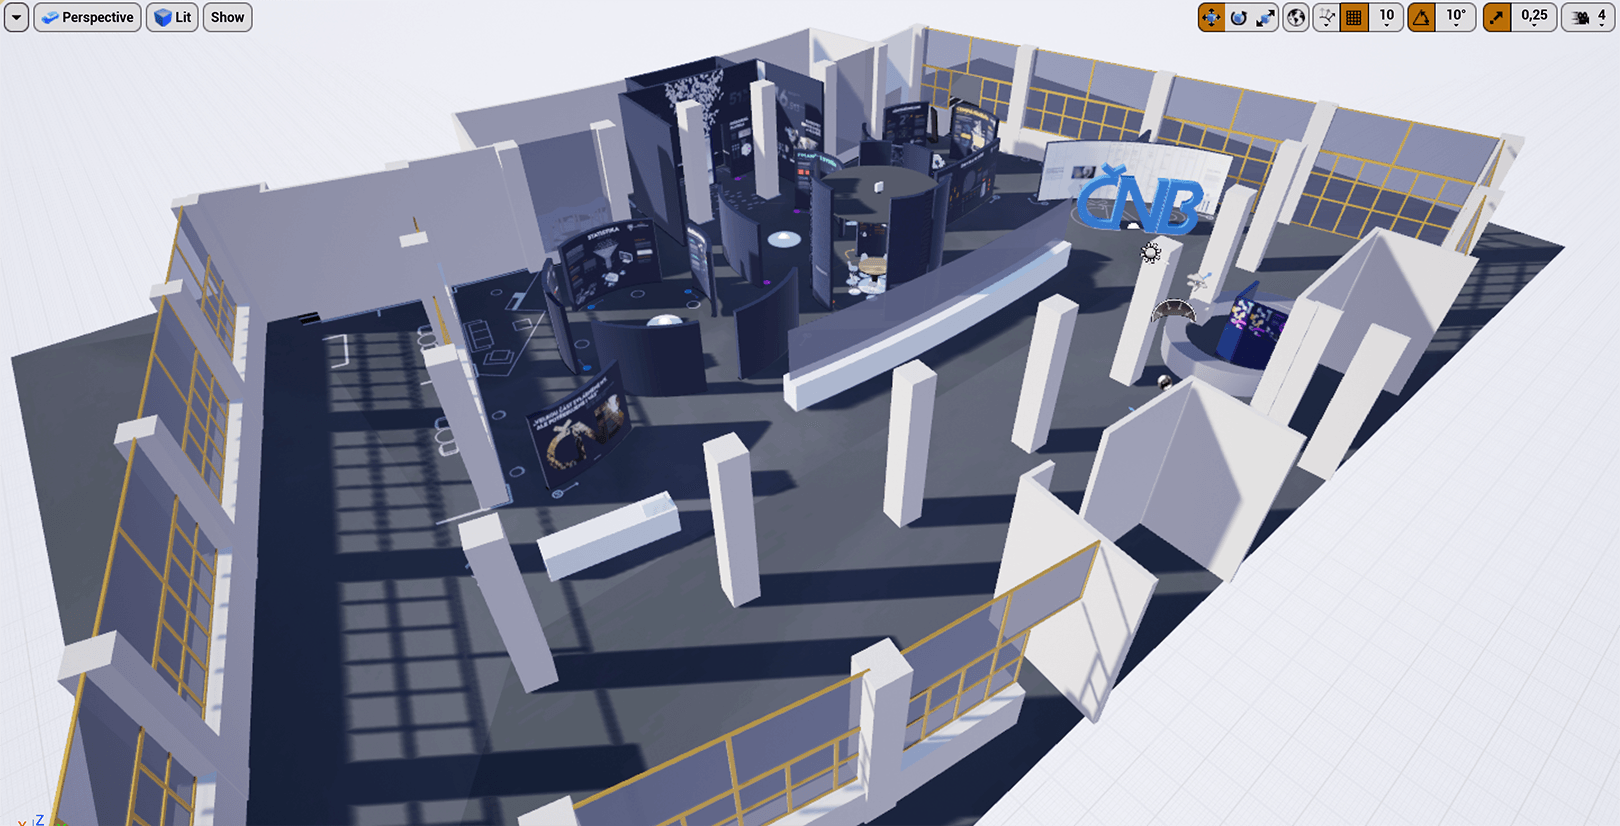
\includegraphics[width=\textwidth]{img/unreal-cnb-scene.png}
    \caption{NC\_ET Level of CNB\_NC\_ET Unreal project.}
    \label{fig:unreal-cnb-level}
\end{figure}

\pagebreak{}
\subsection{Czech National Bank Visitor Centre}
The~scene produced for the~ET experiment is a~Visitor Centre exhibition at the~Czech National Bank~\cite{cnb-nc}. AV MEDIA SYSTEMS, a.s., which was part of this project, internally created a~model of this exhibition in Blender for prototyping purposes~\cite{cnb3dmodel}, the~model can be seen in Figure~\ref{fig:blender-cnb-level}. This prototype was not involved as part of the~construction process. See Figure~\ref{fig:real-cnb-level} where the~exhibition can be seen in a~construction process. Ahrend,~a.s. was responsible for the~realisation of this exhibition in cooperation with AV MEDIA SYSTEMS,~a.s..

\begin{figure}[!ht]\centering
    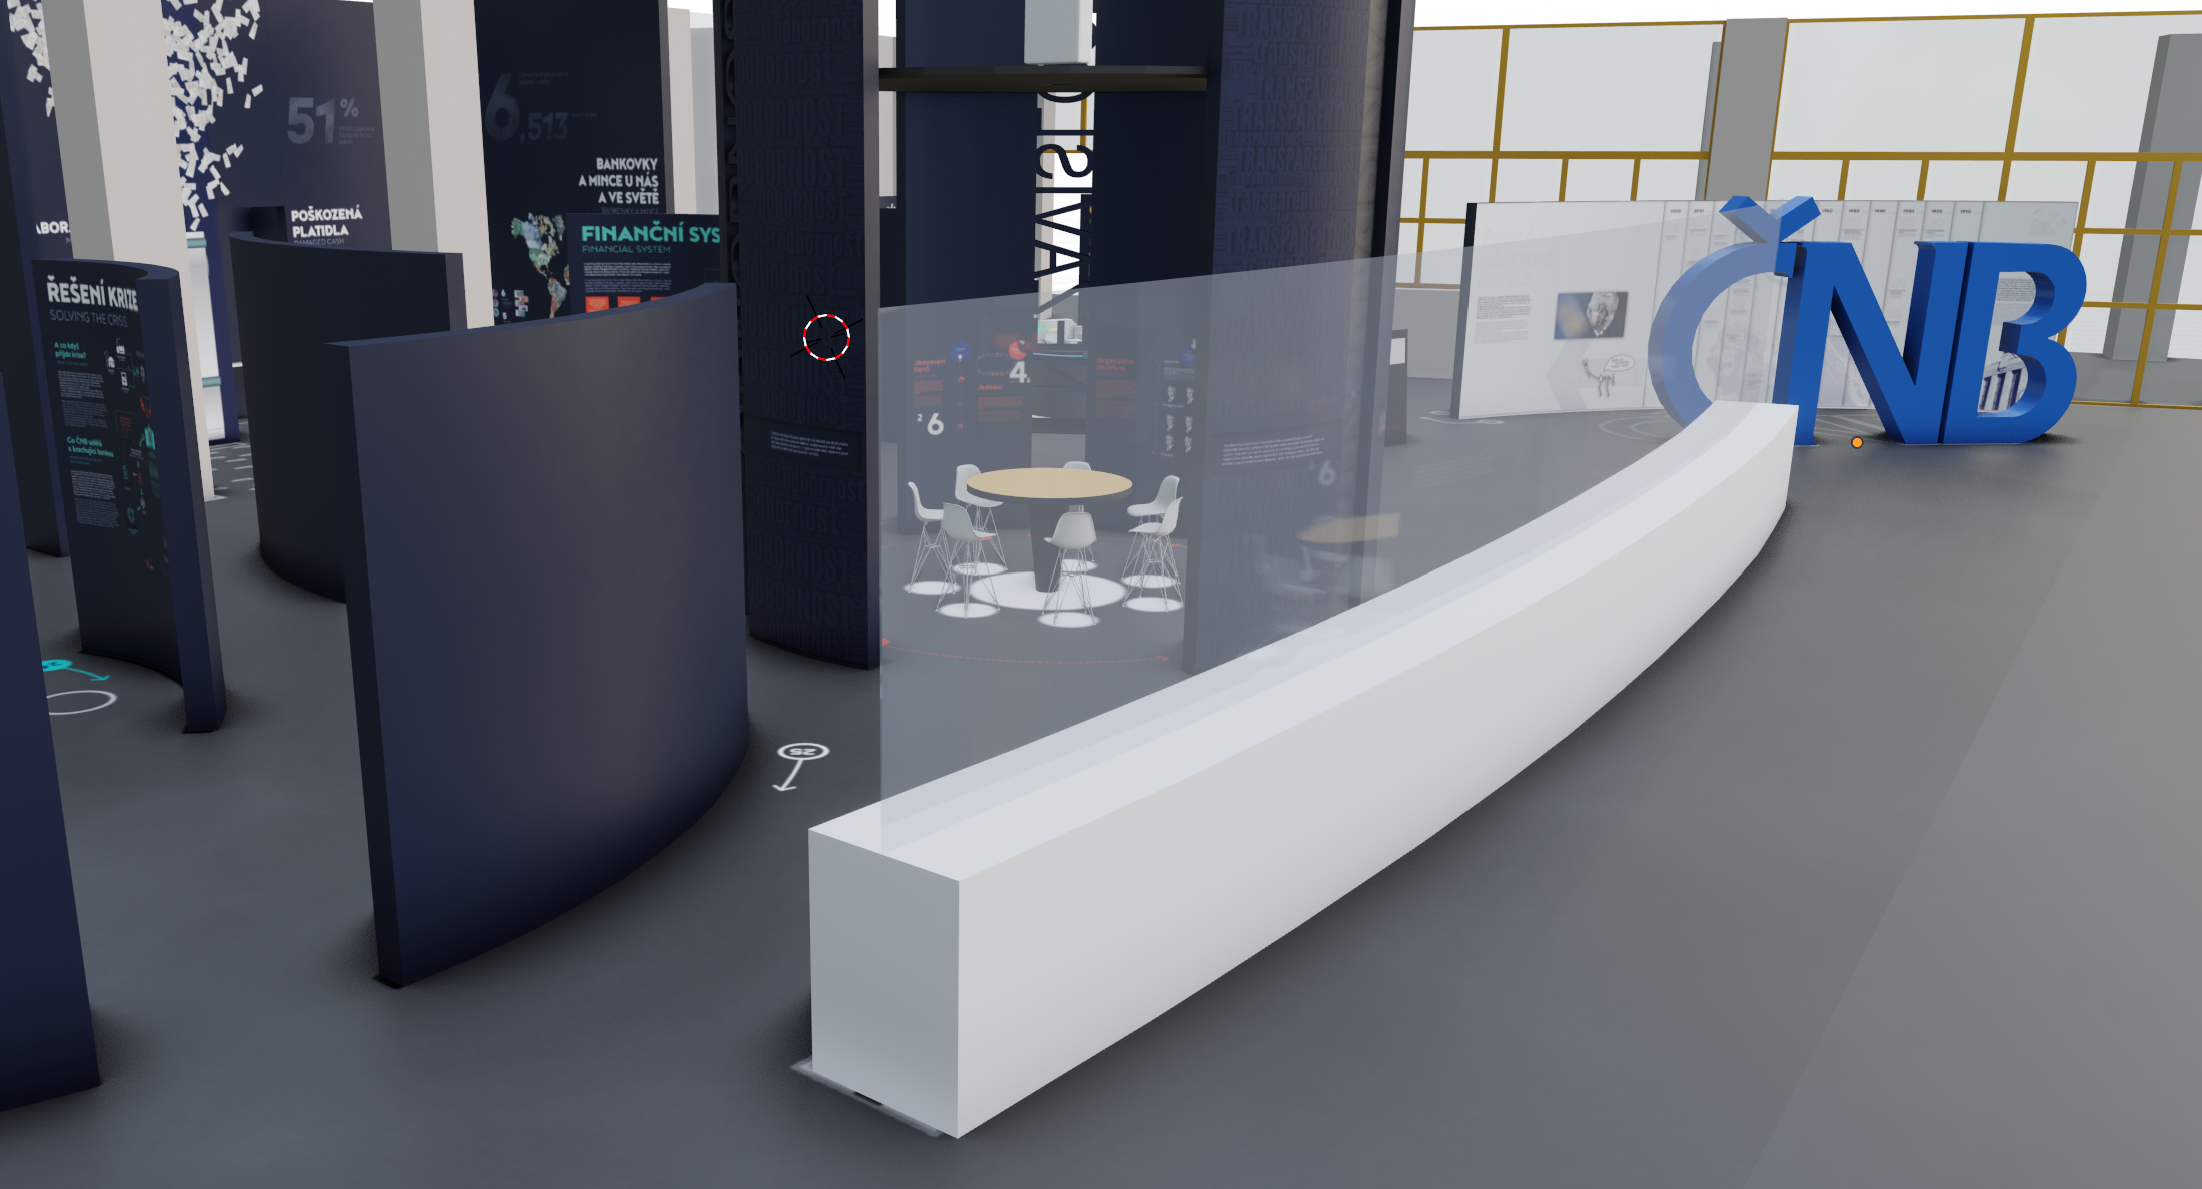
\includegraphics[width=\textwidth]{img/blender-cnb-scene.png}
    \caption[AV MEDIA SYSTEMS, a.s. internal prototype Blender model of CNB Visitor Centre.]{AV MEDIA SYSTEMS, a.s. internal prototype Blender model of CNB Visitor Centre.~\cite{cnb3dmodel}}
    \label{fig:blender-cnb-level}
\end{figure}

\begin{figure}[!ht]\centering
    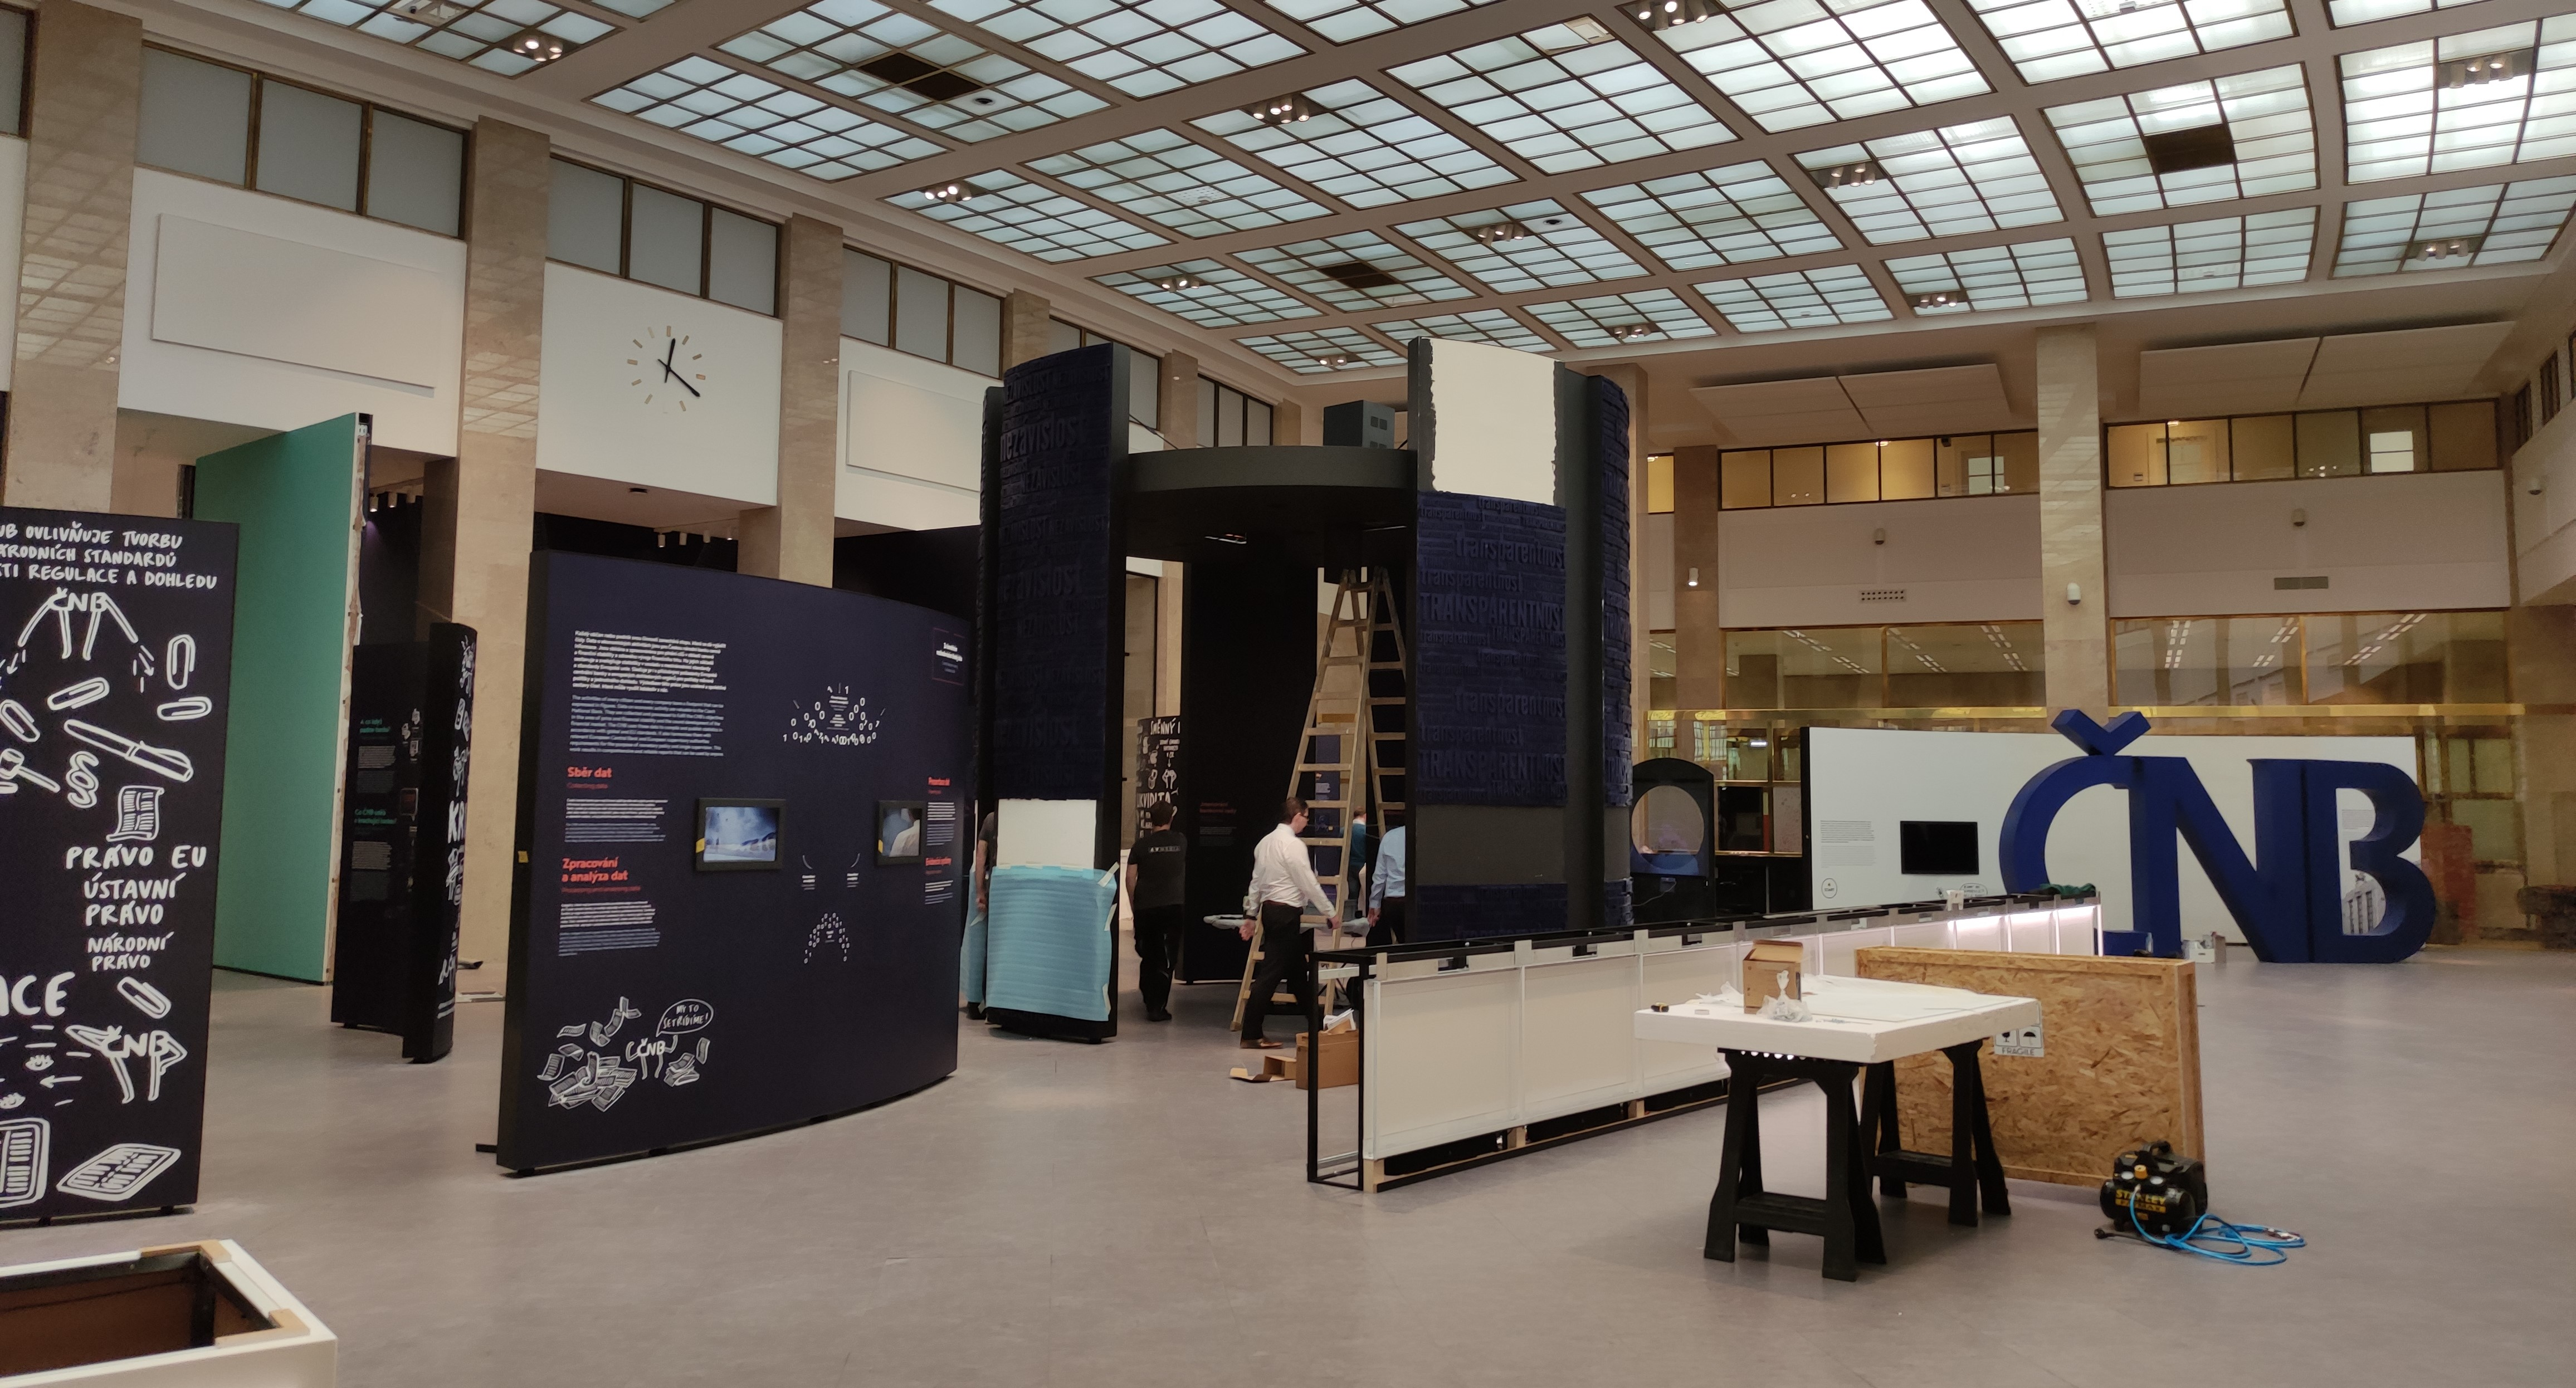
\includegraphics[width=\textwidth]{img/real-cnb-scene.jpg}
    \caption{Visitor Centre of Czech National Bank during construction.}
    \label{fig:real-cnb-level}
\end{figure}

\section{Scene modification}
The~way the~Unreal Engine requires the~definition of objects in levels along with the~definition of the~functionality of the~created plug-in, it would be impractical to convert this model to the~Unreal scene in its original state. This section defines issues with the~Blender scene, which will be modified to allow the~scene to be converted into an~Unreal project~\cite{blender-doc}. The~very first aspect that had to be modified was to separate large models with disconnected meshes into multiple models with their respective material. The~walls and information panels are joined, as illustrated in Figure~\ref{fig:blender-joined-objects}. And the~second problem with most objects in the~scene, as can be seen in Figure~\ref{fig:blender-overlapping-uv}, was that they had defined overlapping UV maps that contained more than one material. 

\begin{figure}[!ht]\centering
    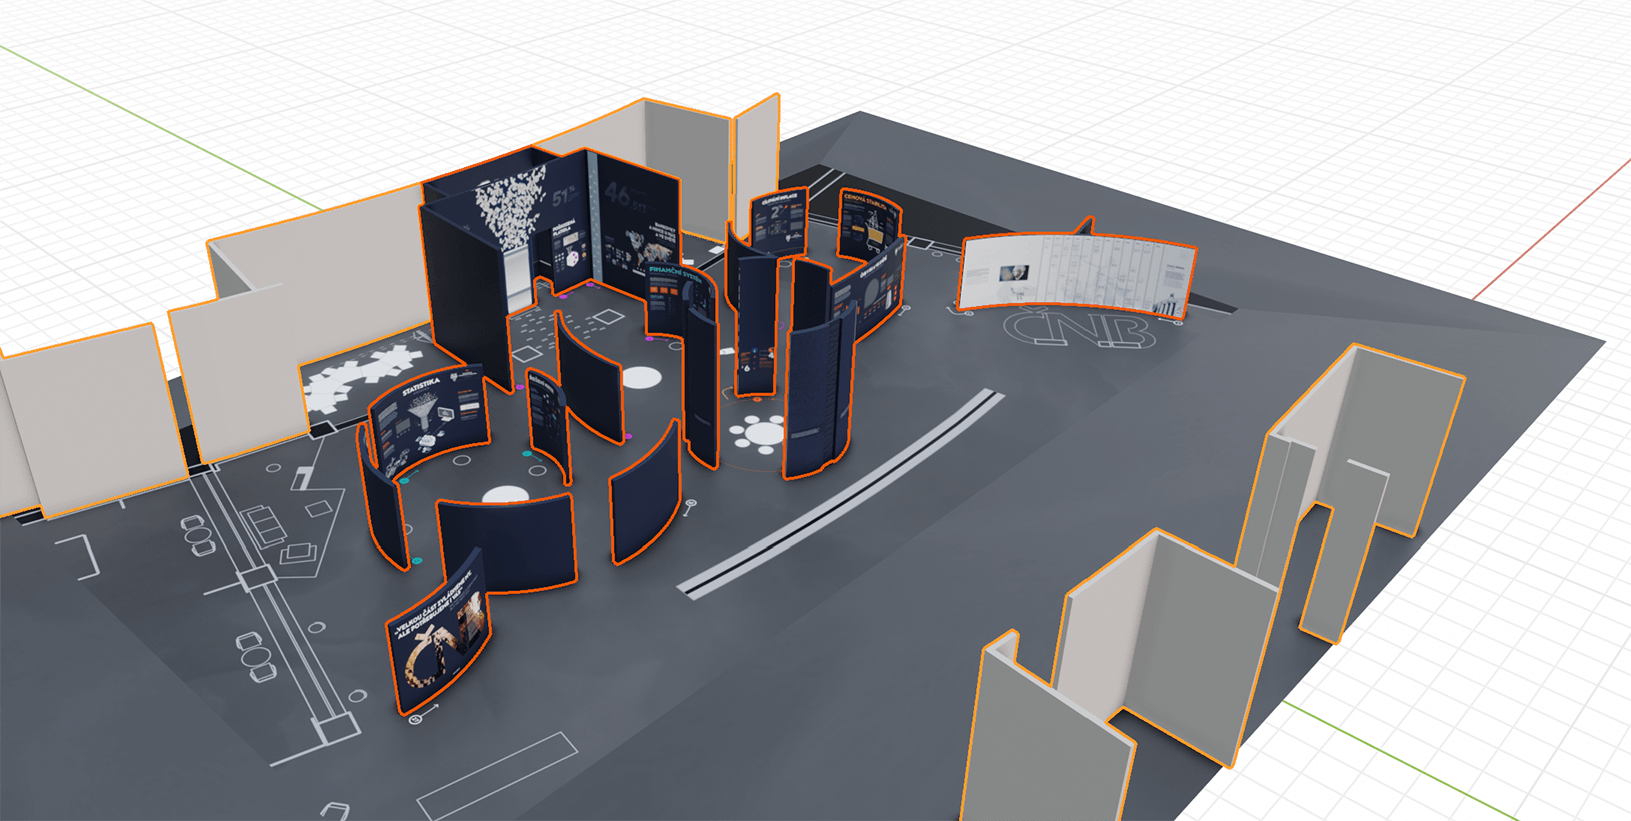
\includegraphics[width=\textwidth]{img/groupped-blender-models.png}
    \caption{Multiple meshes joined into one model.}
    \label{fig:blender-joined-objects}
\end{figure}

\begin{figure}[!ht]\centering
    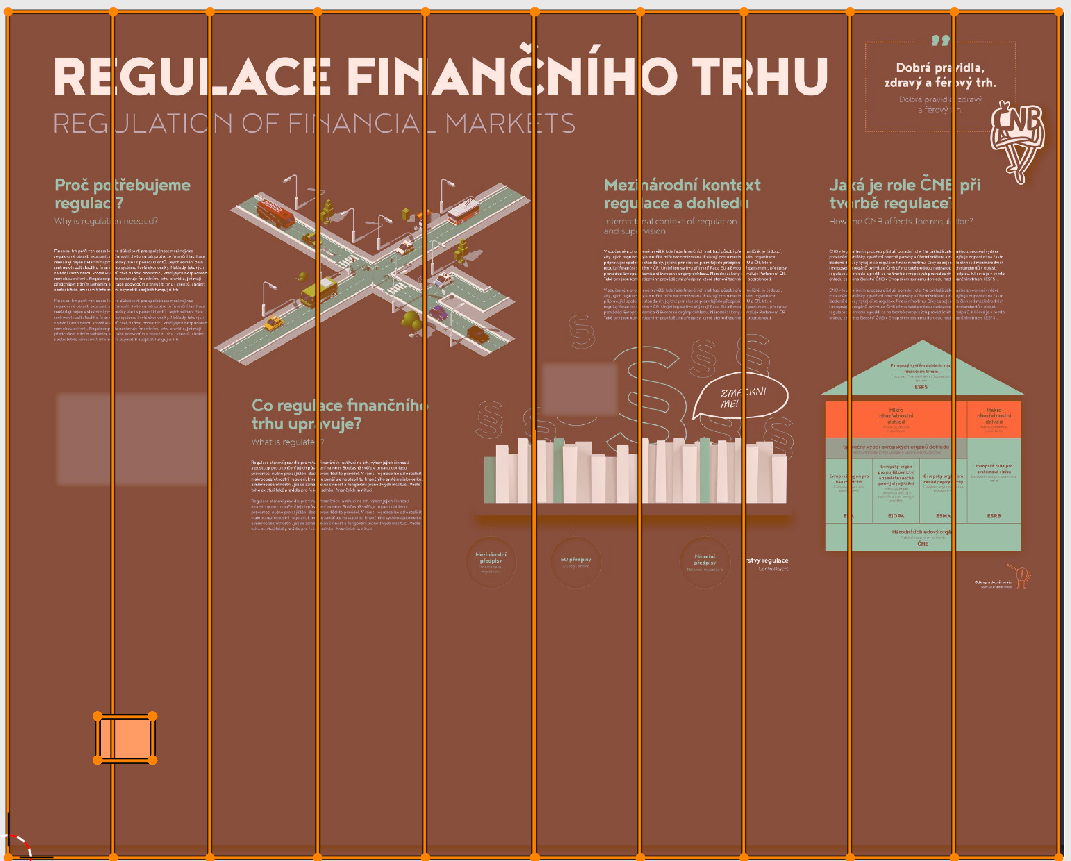
\includegraphics[width=0.55\textwidth]{img/blender-overlapping-uv.png}
    \caption{An~overlapping UV map on one information panel.}
    \label{fig:blender-overlapping-uv}
\end{figure}

\subsection{Joined objects}
The~edit mode had to select all surfaces to be separated from the~shared model and then perform the~operation shown in Figure~\ref{fig:blender-separate-selection}, separate by selection. This object then became independent in the~scene. Next, after this separation, it was worth using the~function again, but this time by material to remove loose material definitions left over from the~other meshes. This was done for all whole meshes in the~model.

Each information panel was defined by two materials. There was always a~material that displayed the~information on a~panel, but there was also a~material that used colour on its back. This colour was defined in panel 2. All the~backs of all the~panels had to be redefined to their own material to match the~original colour from panel 2.

\subsection{Overlapping UVs}
When all meshes are separate, it is important to ensure that heatmaps can be created on these objects according to the~algorithm in Section~\ref{sec:uv-unwrap-method}. It is necessary that these objects have non-overlapping UV maps defined to guarantee uniqueness for all mesh faces.

This is done in the~Object Data Properties setting of the~object. A~new map is added in the~UV Maps section and it is important to keep the~original one for the~next step. This new UV map can be defined using a~Blender feature in edit mode called Smart UV Project, which will generate the~UV map itself according to the~specified parameters. However, it is not recommended to do this without first manually defining seam edges, as, for some objects, this automatic generation could potentially yield poor results. Marking an~edge as a~seam can be seen in Figure~\ref{fig:blender-mark-seam}.

Some objects capable of being in the~Unreal project with the~plug-in have no UV maps defined or use a~basic material. These are simpler cases for which a~definition of a~new UV map is sufficient. 

\begin{figure}[!b]\centering
    \begin{subfigure}[b]{0.47\textwidth}
        \centering
        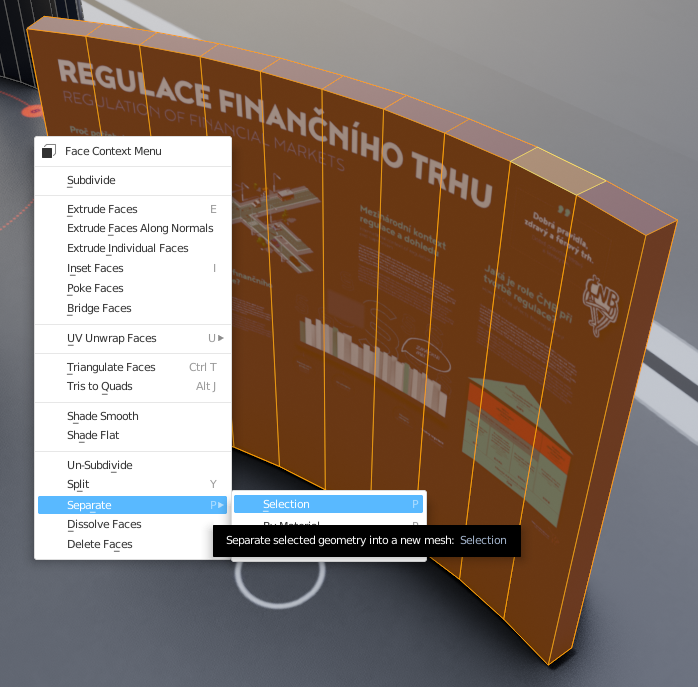
\includegraphics[width=\textwidth]{img/blender-separate-selection.png}
        \caption{Separate selection of faces into new mesh.}
        \label{fig:blender-separate-selection}
    \end{subfigure}
    \hfill
    \begin{subfigure}[b]{0.52\textwidth}
        \centering
        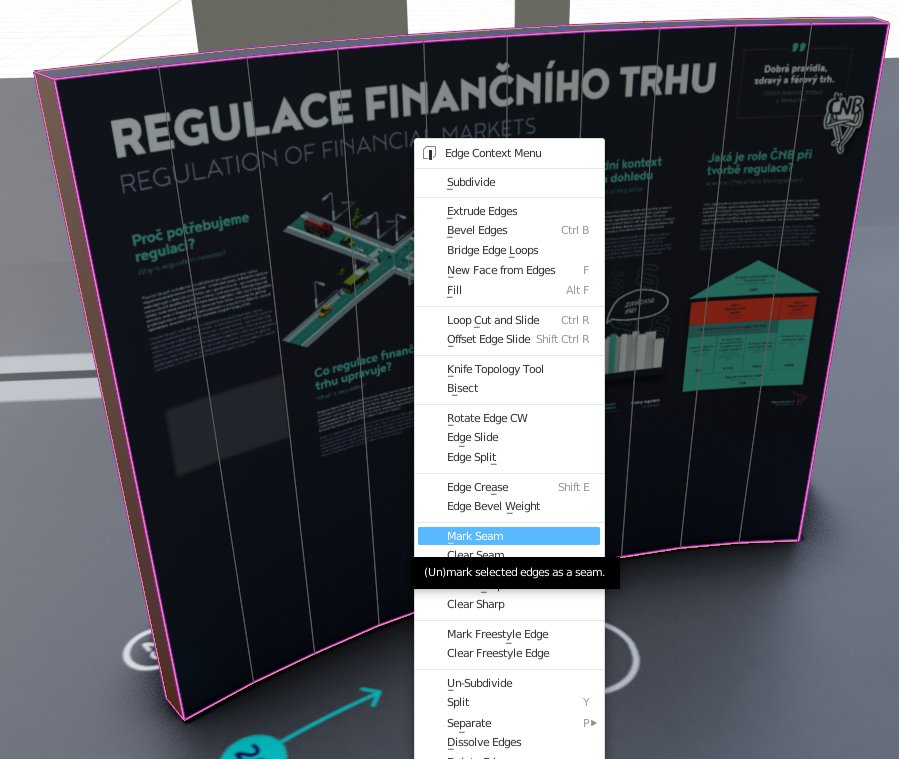
\includegraphics[width=\textwidth]{img/blender-mark-seam.png}
        \caption{Mark mesh edges as seam for UV unwrap.}
        \label{fig:blender-mark-seam}
    \end{subfigure}
    \caption{Blender edit mode separate selection and mark seam operations.}
\end{figure}

\pagebreak{}
\subsection{Material Baking}
This step describes the~Blender procedure to convert a~material defined for one UV map to another using texture baking. Also described in this tutorial~\cite{blender-texture-baking-tutorial}.

The~method consists of defining a~new UV map on the~same object. The~complete setup can be seen in Figure~\ref{fig:blender-bake-nodes}. Then, in the~Shader Editor, add a~new \emph{ImageTexture} material node through which a~new texture is created without an~alpha channel of square resolution. This node is connected to the~material node \emph{UV Map}, which links to the~newly created \emph{UVMapBake}. To be absolutely sure, the~original UV map can be linked to the~original texture.

\begin{figure}[!ht]\centering
    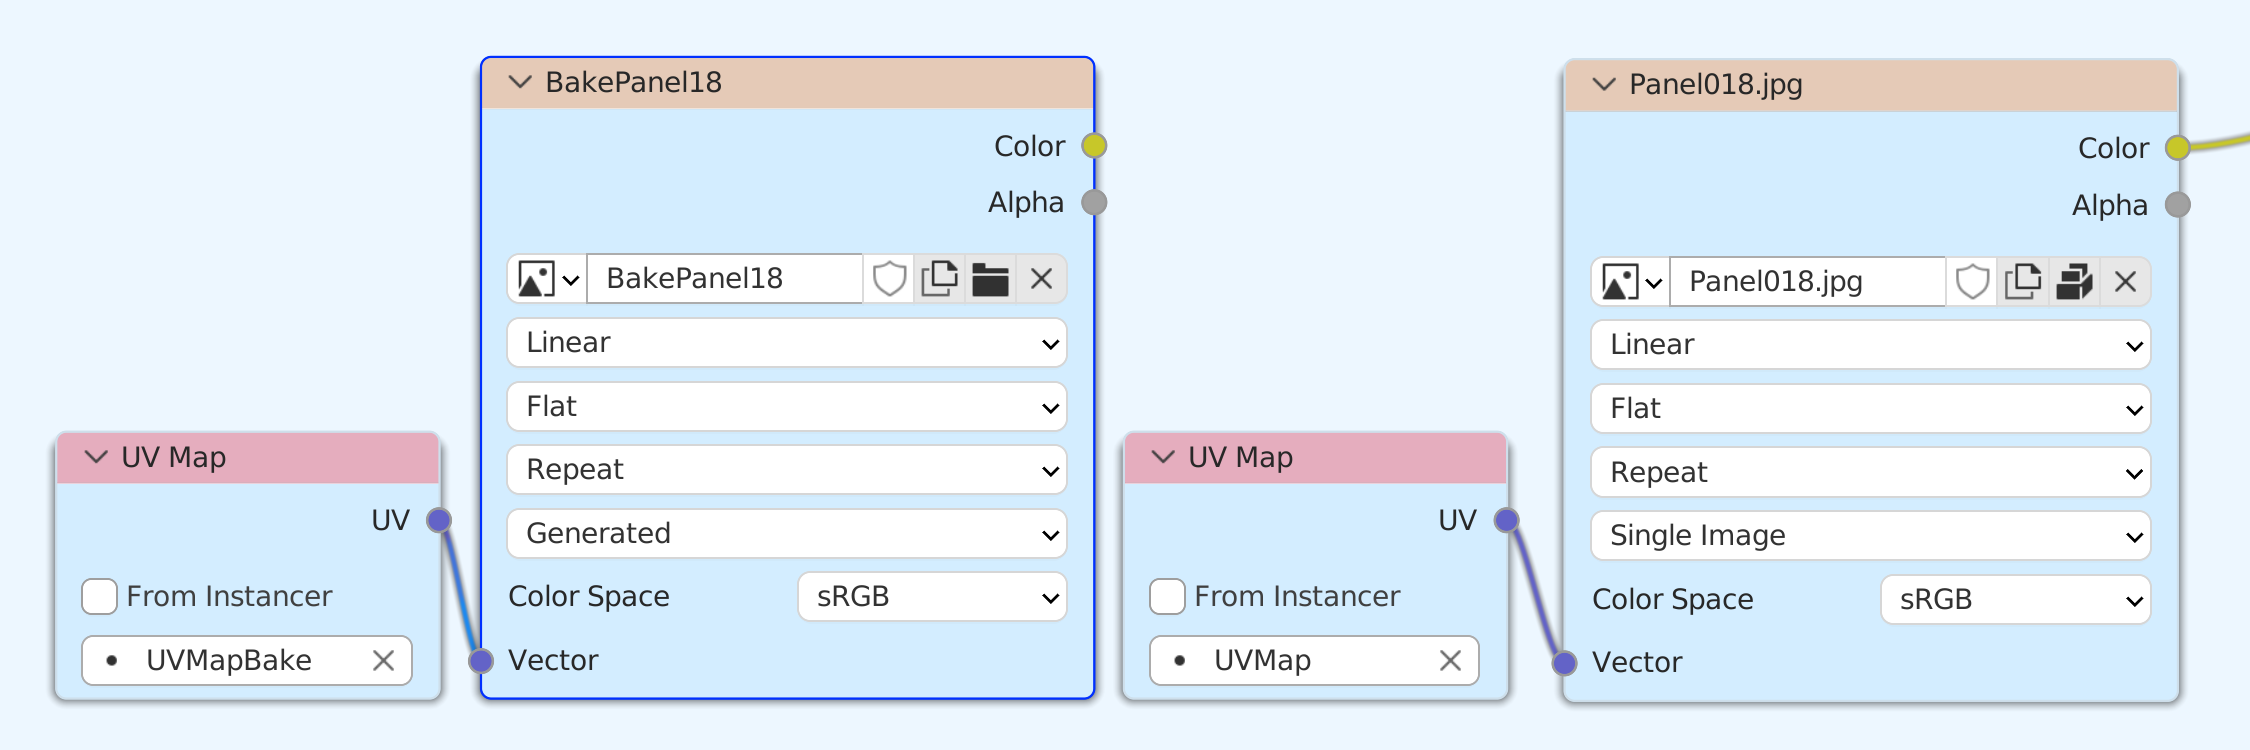
\includegraphics[width=\textwidth]{img/blender-bake-nodes.png}
    \caption{Preparation of the~information panel material nodes for baking into a~new texture.}
    \label{fig:blender-bake-nodes}
\end{figure}

To bake into UVMapBake, it is necessary to open the~Bake settings of Blender's Cycles renderer and select the~corresponding ImageTexture node. Cycles settings are in Figure~\ref{fig:blender-bake-settings}. It is enough to set the~diffuse \emph{BakeType} that will not include direct or indirect light from the~scene, only colour. The~resulting texture can be saved or embedded in the~project. The~difference between the~baked texture and the~original texture can be seen in the~Appendix~\ref{appendix:baked-textures}.

\begin{figure}[!ht]\centering
    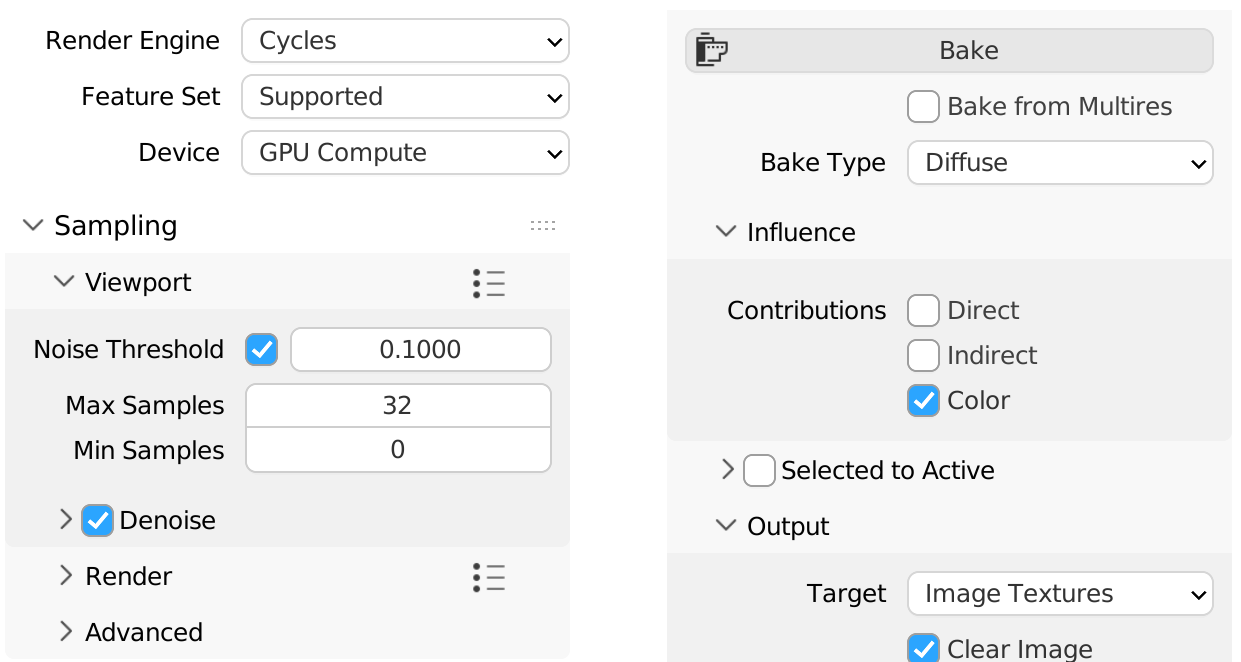
\includegraphics[width=\textwidth]{img/blender-bake-settings.png}
    \caption{Blender cycles settings for baking simple diffuse colour onto an~ImageTexture.}
    \label{fig:blender-bake-settings}
\end{figure}

\subsection{Origin of models}
\label{sec:blender-origins}
The~original model contains many grouped objects that share a~common origin or have their origin right at the~origin of the~scene. This needs to be changed for those objects that will be exported, due to Unreal Engine's rendering pipeline, which culls in one step those objects that are not visible in the~view frustum. This happens during heatmap rendering when the~object is somewhere else than where the~Scene Capture Component is looking. Section~\ref{sec:uv-unwrap-implementation} describes how the~render Actor changes its position in the~world based on the~position of the~object being rendered. Because of this, the~mesh itself must be guaranteed to be near its origin for at least the~distance determined by the~size of the~rendered heatmap texture, which also determines the~width of the~orthographic frustum.

In Blender, it is worth setting the~length of the~units to centimetres in Scene Properties first to mimic the~unit system in Unreal. Origin can be changed in the~context of this scene in the~following style; generate a~new origin at the~centre of the~object geometry, place a~3D cursor on this new origin and set the~z-coordinate to 0 so the~cursor will sit on the~ground, and finally assign the~object's origin to this 3D cursor.

\subsection{Model export}

An~object with a~newly defined UV map, a~material that contains the~newly baked texture of the~original material, can be exported to Unreal Engine. It includes tools that allow some 3D modelling programmes to export their entire scenes at once. This is called \emph{Datasmith}. This was only available in the~past using an~unofficial Blender plug-in, which was not supported and could not be used at the~time of writing the~thesis. This route cannot be taken; the~conversion of the~whole scene is done manually.

Exporting an~object from Blender as an~\path{.fbx} file allows one to bundle its mesh, material, and texture with it. Procedural materials cannot be exported in this manner and must be baked before.

\section{Unreal project}
This section will describe how the~experiment scene was constructed by adding exported models one by one from Blender. The~entire project can be found in the~enclosed media in.

\subsection{Setting up the~scene}
The~models were inserted into the~scene inside the~logical entities represented by different Actors in the~project directory in the~Map folder, Figure~\ref{fig:cnb-scene-contents}.

\begin{figure}[!ht]\centering
    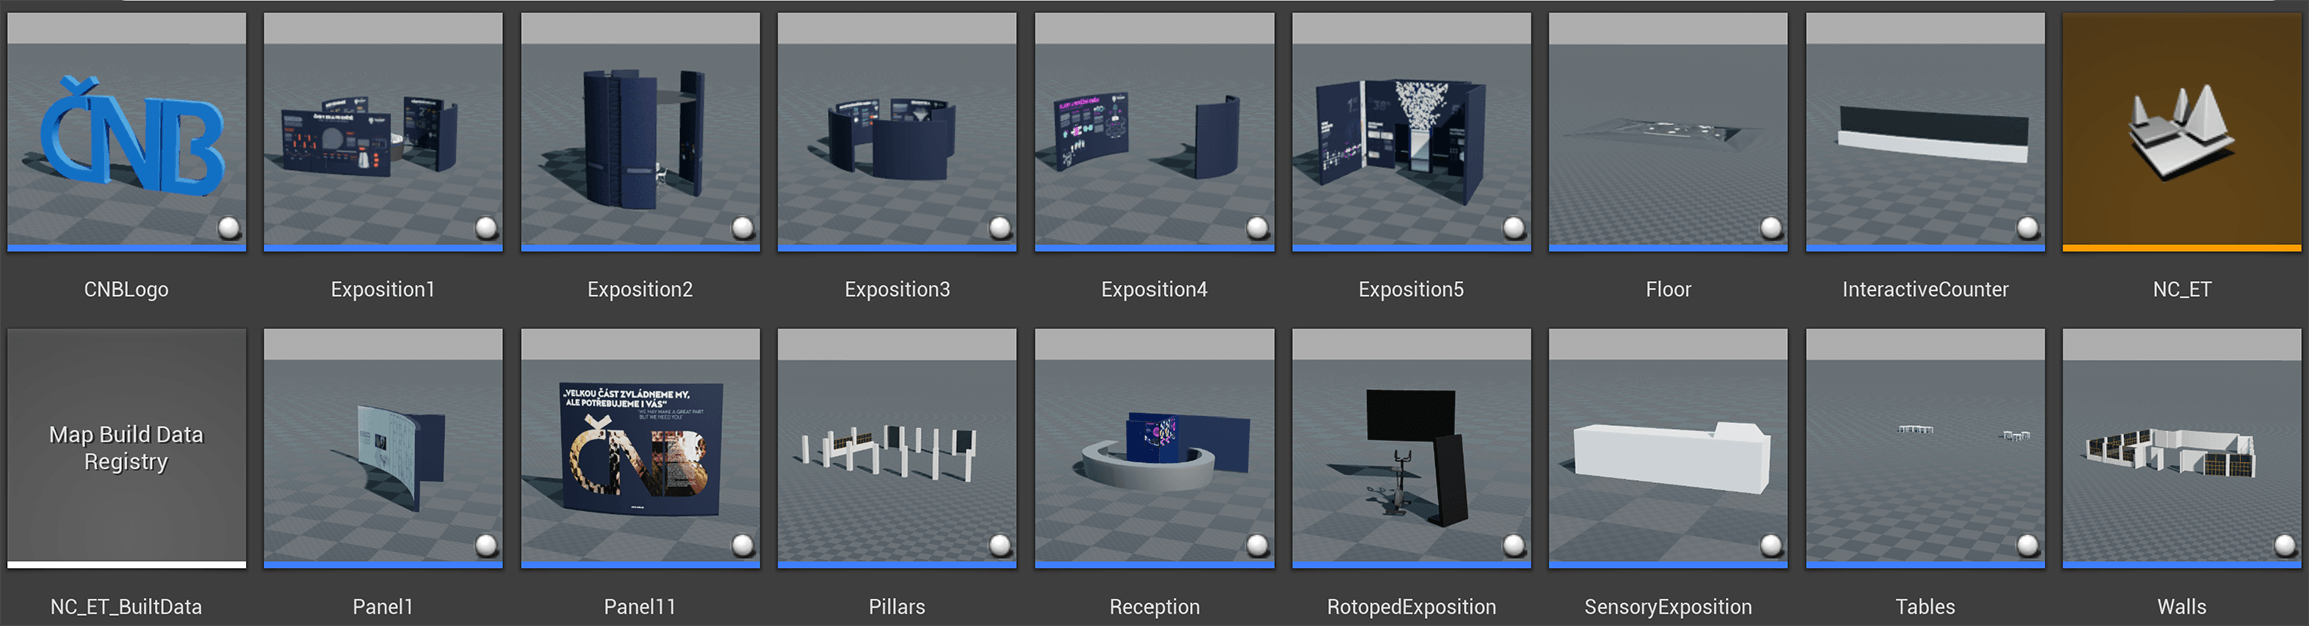
\includegraphics[width=\textwidth]{img/cnb-scene-contents.png}
    \caption{Actors containing scene objects.}
    \label{fig:cnb-scene-contents}
\end{figure}

\subsubsection*{Asset placement}
An~Fbx file can always be imported into Unreal with a~simple drag-and-drop. At most, such an~object brought StaticMesh, Material and Texture2D with it into the~project. These Assets are, respectively, divided into Geometries, Materials, and Textures directories. All imported models are in their local coordinates, guaranteed by setting up their origins according to Section~\ref{sec:blender-origins}.

For a~logical scene entity such as an~exhibit, a~single Actor was used. For this actor, several components of the~EyeTrackedStaticMeshComponent class defined in Section~\ref{sec:static-mesh-ET} were added. Those were manually placed in the~local world coordinate system of a~given Actor exactly according to the~coordinates that the~meshes would have in Blender relative to the~origin of an~exhibit. See Figure~\ref{fig:exhibit-definition}.
Each of these components has been assigned a~StaticMesh. Next, the~texture resolution and the~\emph{AcceptsHeat} boolean are set.

Not all objects from the~scene in Blender were used to keep the~experiment relatively clean. The~reason is the~recording of both heatmaps from the~eye tracker and the~virtual camera. The~simpler one has a~much larger brush radius set, so it is worth demonstrating it on objects that are large.

\begin{figure}[!ht]\centering
    \begin{subfigure}[b]{0.495\textwidth}
        \centering
        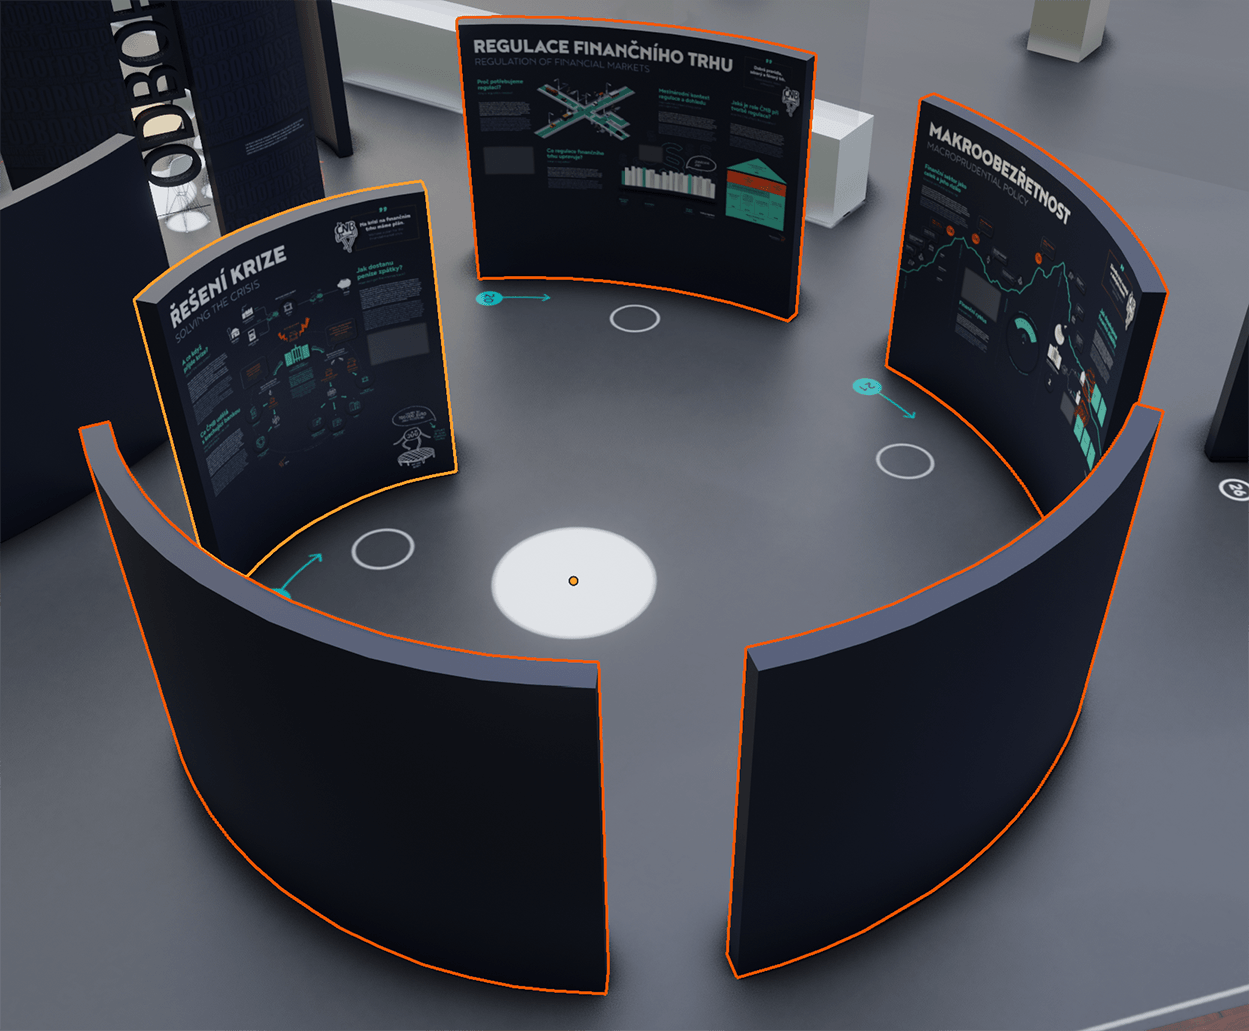
\includegraphics[width=\textwidth]{img/blender-exhibit.png}
        \caption{Panels with origin at exhibit centre in Blender.}
    \end{subfigure}
    \hfill
    \begin{subfigure}[b]{0.495\textwidth}
        \centering
        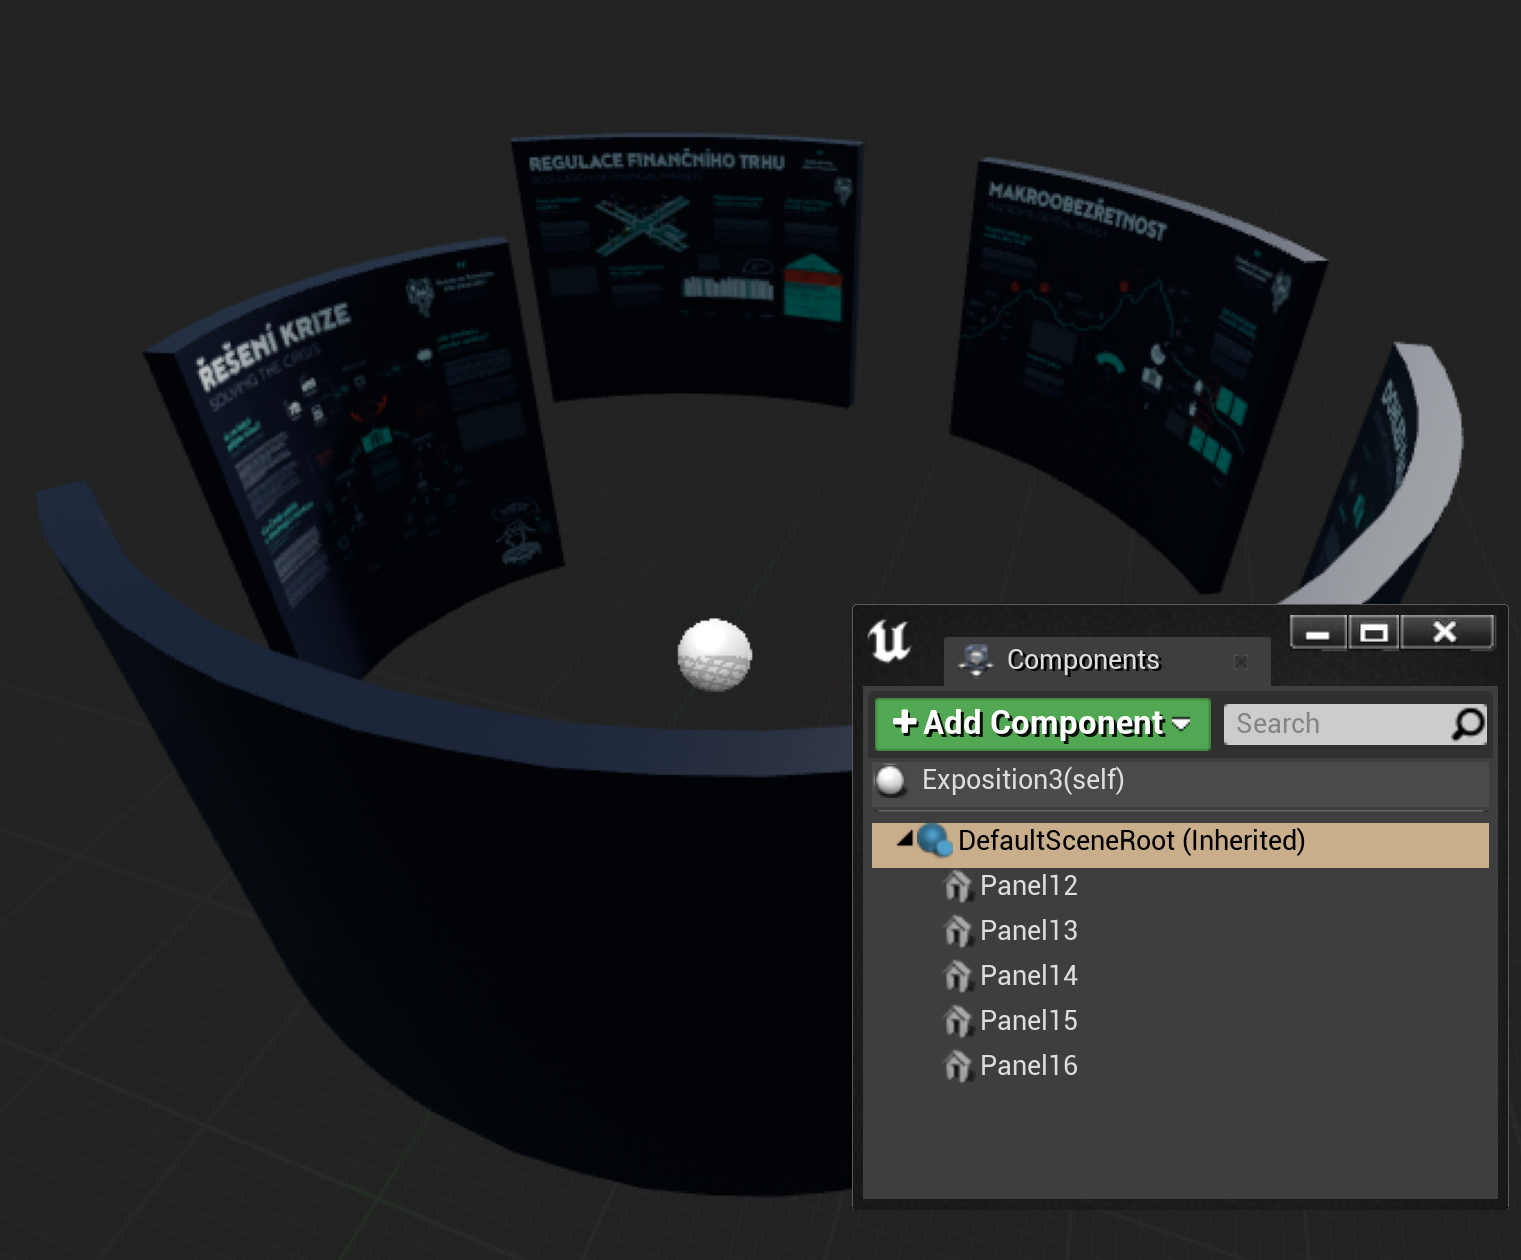
\includegraphics[width=\textwidth]{img/unreal-exhibit.png}
        \caption{Panels defined around Actor's origin in UE.}
    \end{subfigure}
    \caption{Exhibit defined as logical scene entity.}
    \label{fig:exhibit-definition}
\end{figure}

\subsubsection*{Collisions}
Each StaticMesh can be collided with using its complex collision, which is in effect just a~collision against all its faces. It is possible to define simple collisions for the~mesh in the~Static Mesh Editor in Unreal Engine to reduce the~complexity of collision calculations. For all static meshes imported from Blender, the~Convex Decomposition function in the~editor was used to generate a~simple collision volume. 

\pagebreak{}

\subsection{Pawns}
\label{sec:pawns}
In the~scene, two Pawns are defined to move around the~scene. One is used to collect data, while the~other is used only to view them. 

\subsubsection*{VRCollector}
This pawn is a~pure pawn without any movement ability. It contains the~GazeEmitter component described in Section~\ref{sec:gaze-emitter} and a~camera that is directly locked to an~absolute HMD position obtained from a~positioning system. The~problem with these coordinates is that they do not move with a~pawn in the~world; they move with it. To keep them positioned in the~same way as the~camera, it is necessary to fix the~pawn at the~origin of the~world from which it will not move. To solve this problem, the~pawn will not traverse the~scene, but the~entire scene will move around the~pawn. Specifically, in the~opposite direction to the~way the~pawn wants to move. See Figure~\ref{fig:vr-pawn-movement}. In the~whole scene, an~Actor \emph{SceneOrigin} has been created who is superior to all other Actors. 


Its main functionality, however, is that it starts an~experiment that lasts three minutes. When finished, all textures are saved in the~folder \path{C:/ProgramData/NC_ET/} and the~programme is exited, as can be seen in Figure~\ref{fig:experiment-definition}. During this experiment, data were collected using the~GazeEmitter component, Section~\ref{sec:gaze-emitter}. Figure~\ref{fig:heatmap-rendering-cycle} shows the~Tick Event of this Pawn, which always asks if the~experiment is running. If it does, it sends the~forward vector of the~Camera from its origin as a~ray classified as Camera ray type to the~\emph{Emit Ray From} function, defined in Section~\ref{sec:gaze-emitter}. It can also be seen in the~figure that the~same vector is sent for the~ray classified as Gaze. The~reason for this is discussed in Section~\ref{sec:data-collection}. The~implementation of this cycle corresponds exactly to the~activity diagram in Figure~\ref{fig:experiment-diagram} in Section~\ref{sec:plugin-functionality}.

\begin{figure}[!ht]\centering
    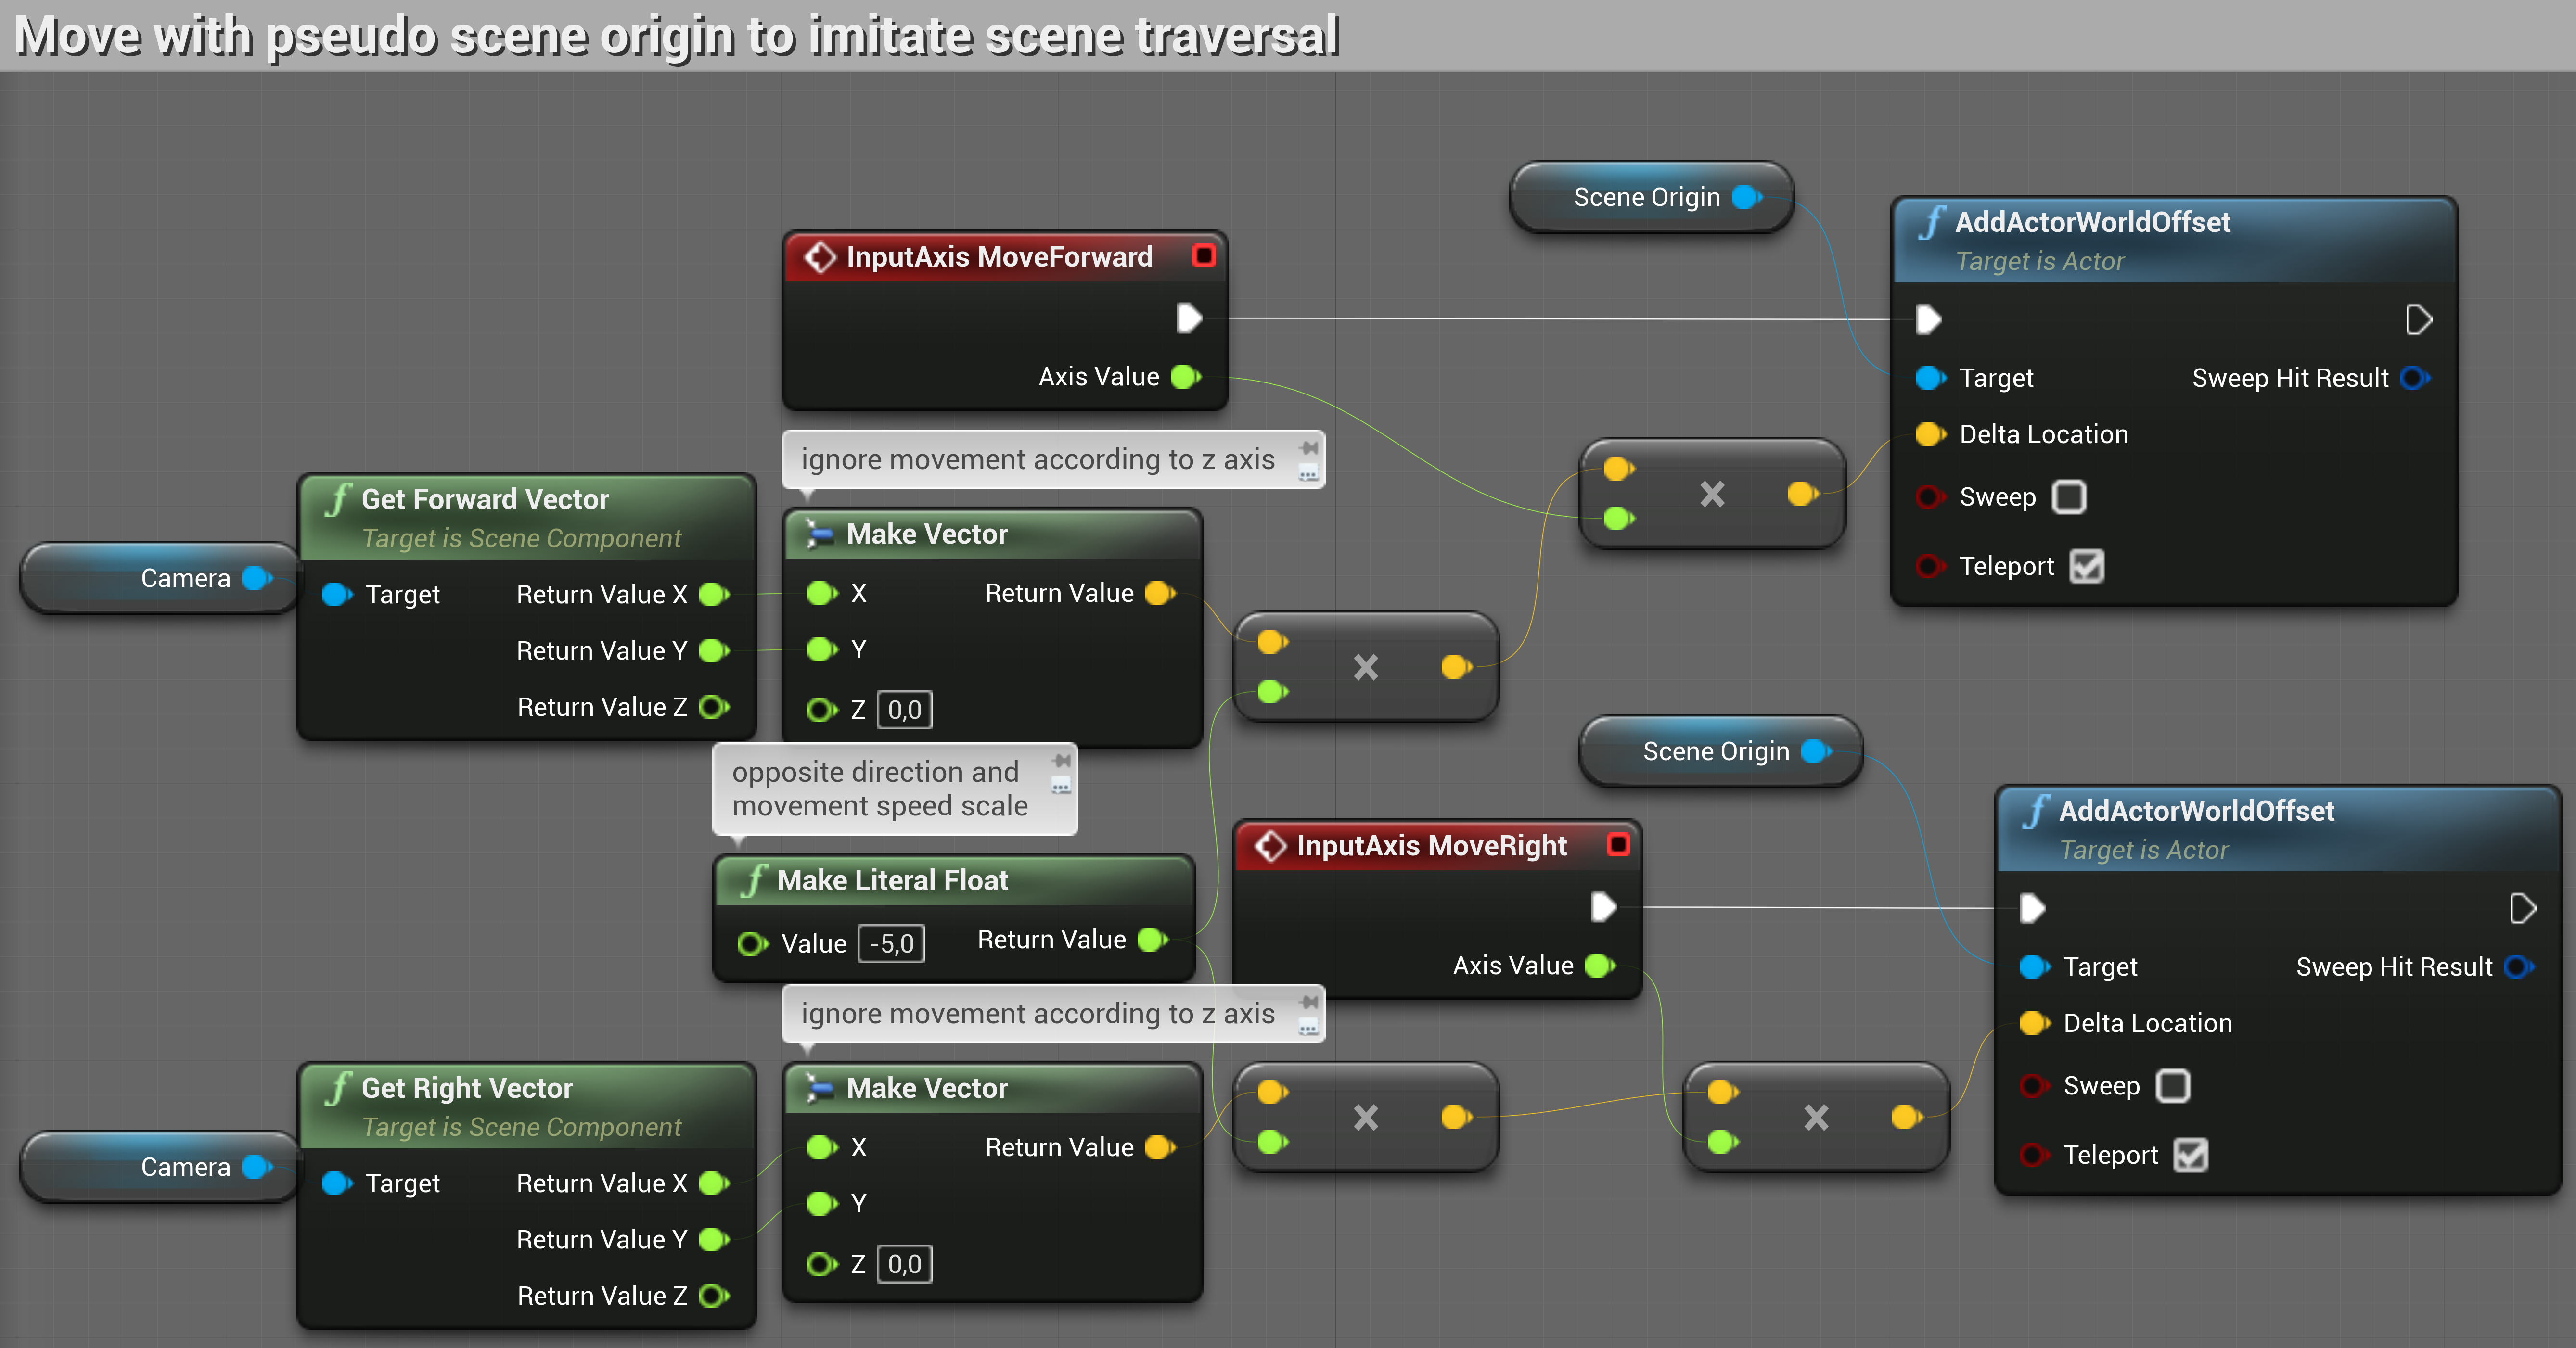
\includegraphics[width=\textwidth]{img/vr-pawn-movement.png}
    \caption{VRCollector movement definition.}
    \label{fig:vr-pawn-movement}
\end{figure}

\pagebreak{}

\begin{figure}[!ht]\centering
    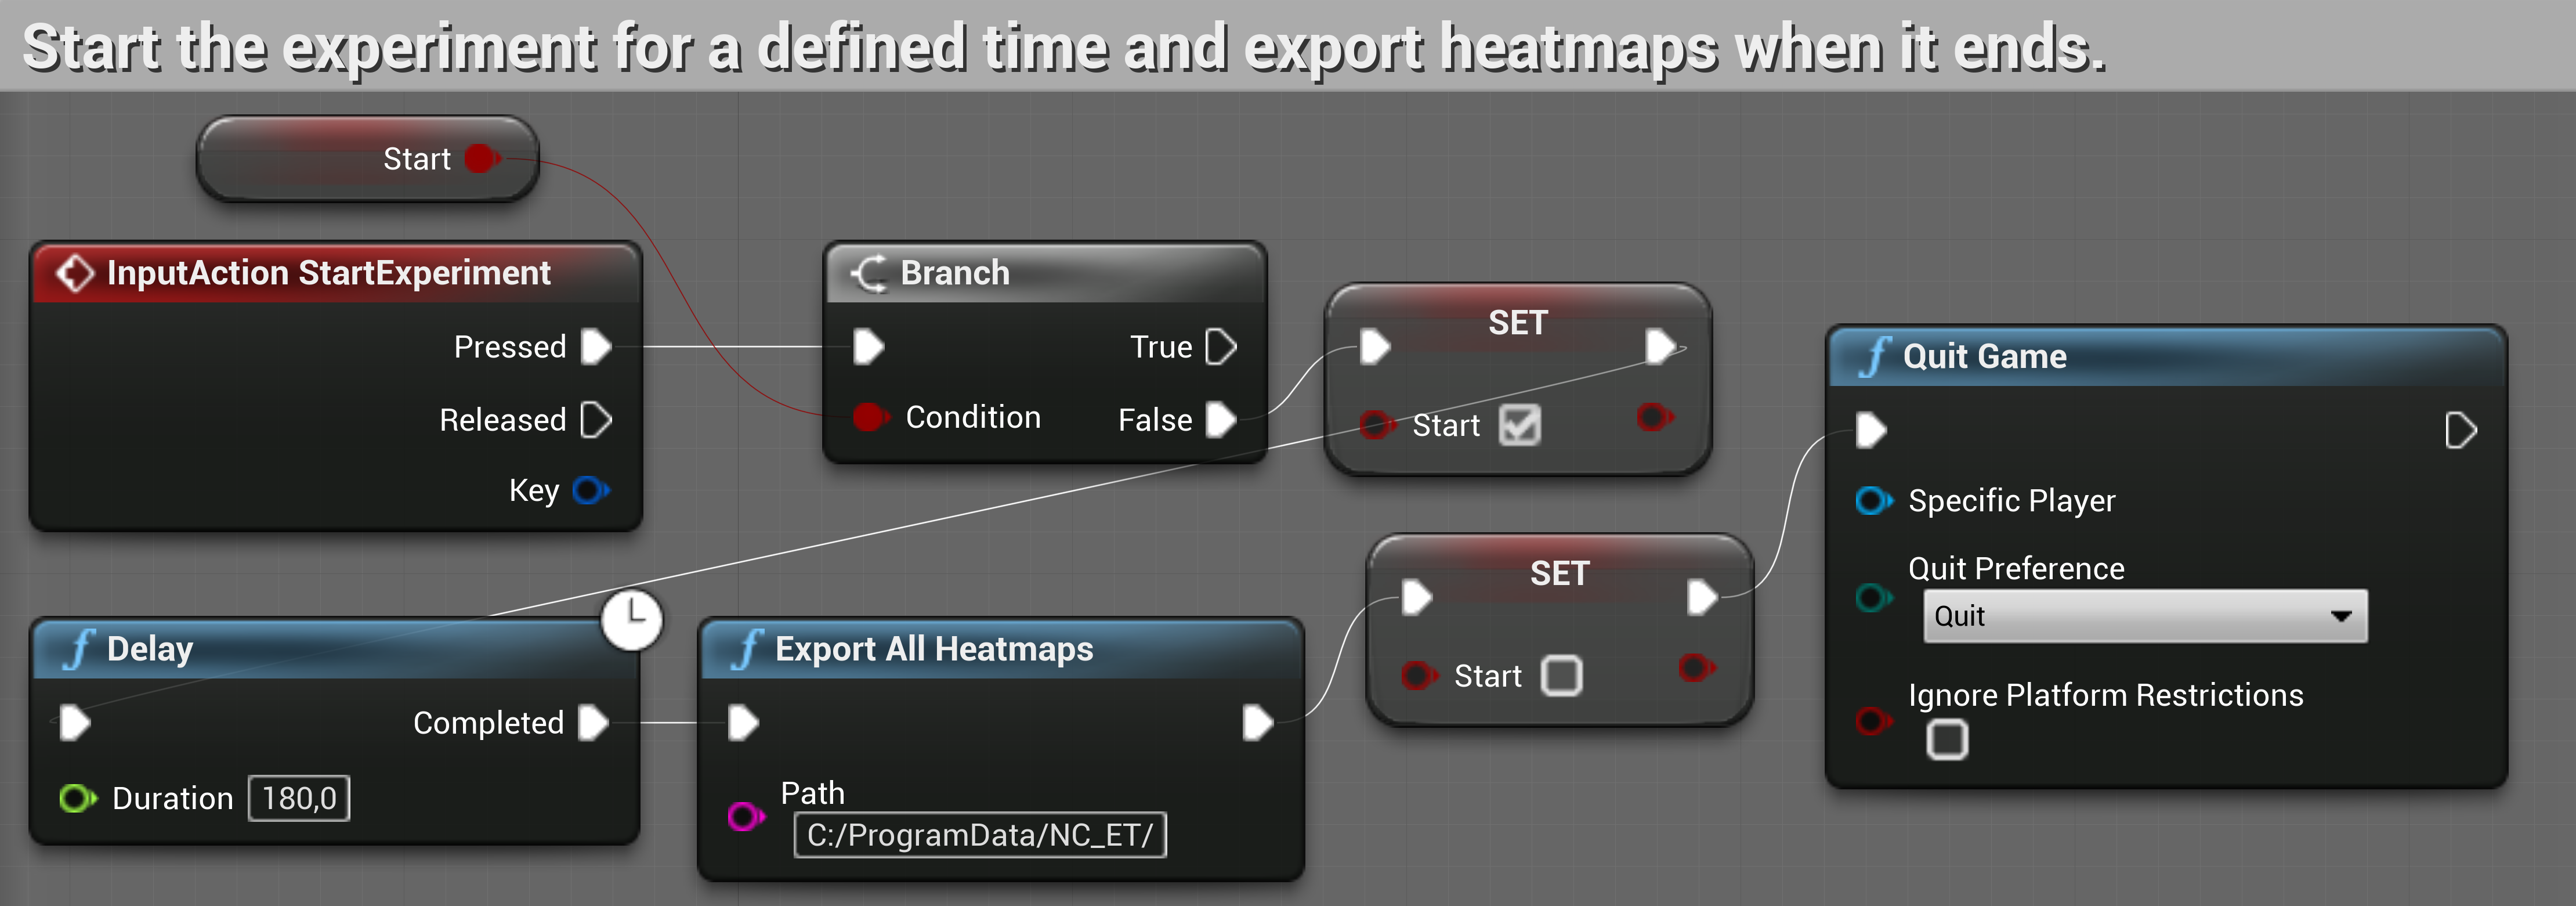
\includegraphics[width=\textwidth]{img/experiment-definition.png}
    \caption{VRCollector set experiment start and duration.}
    \label{fig:experiment-definition}
\end{figure}

\begin{figure}[!ht]\centering
    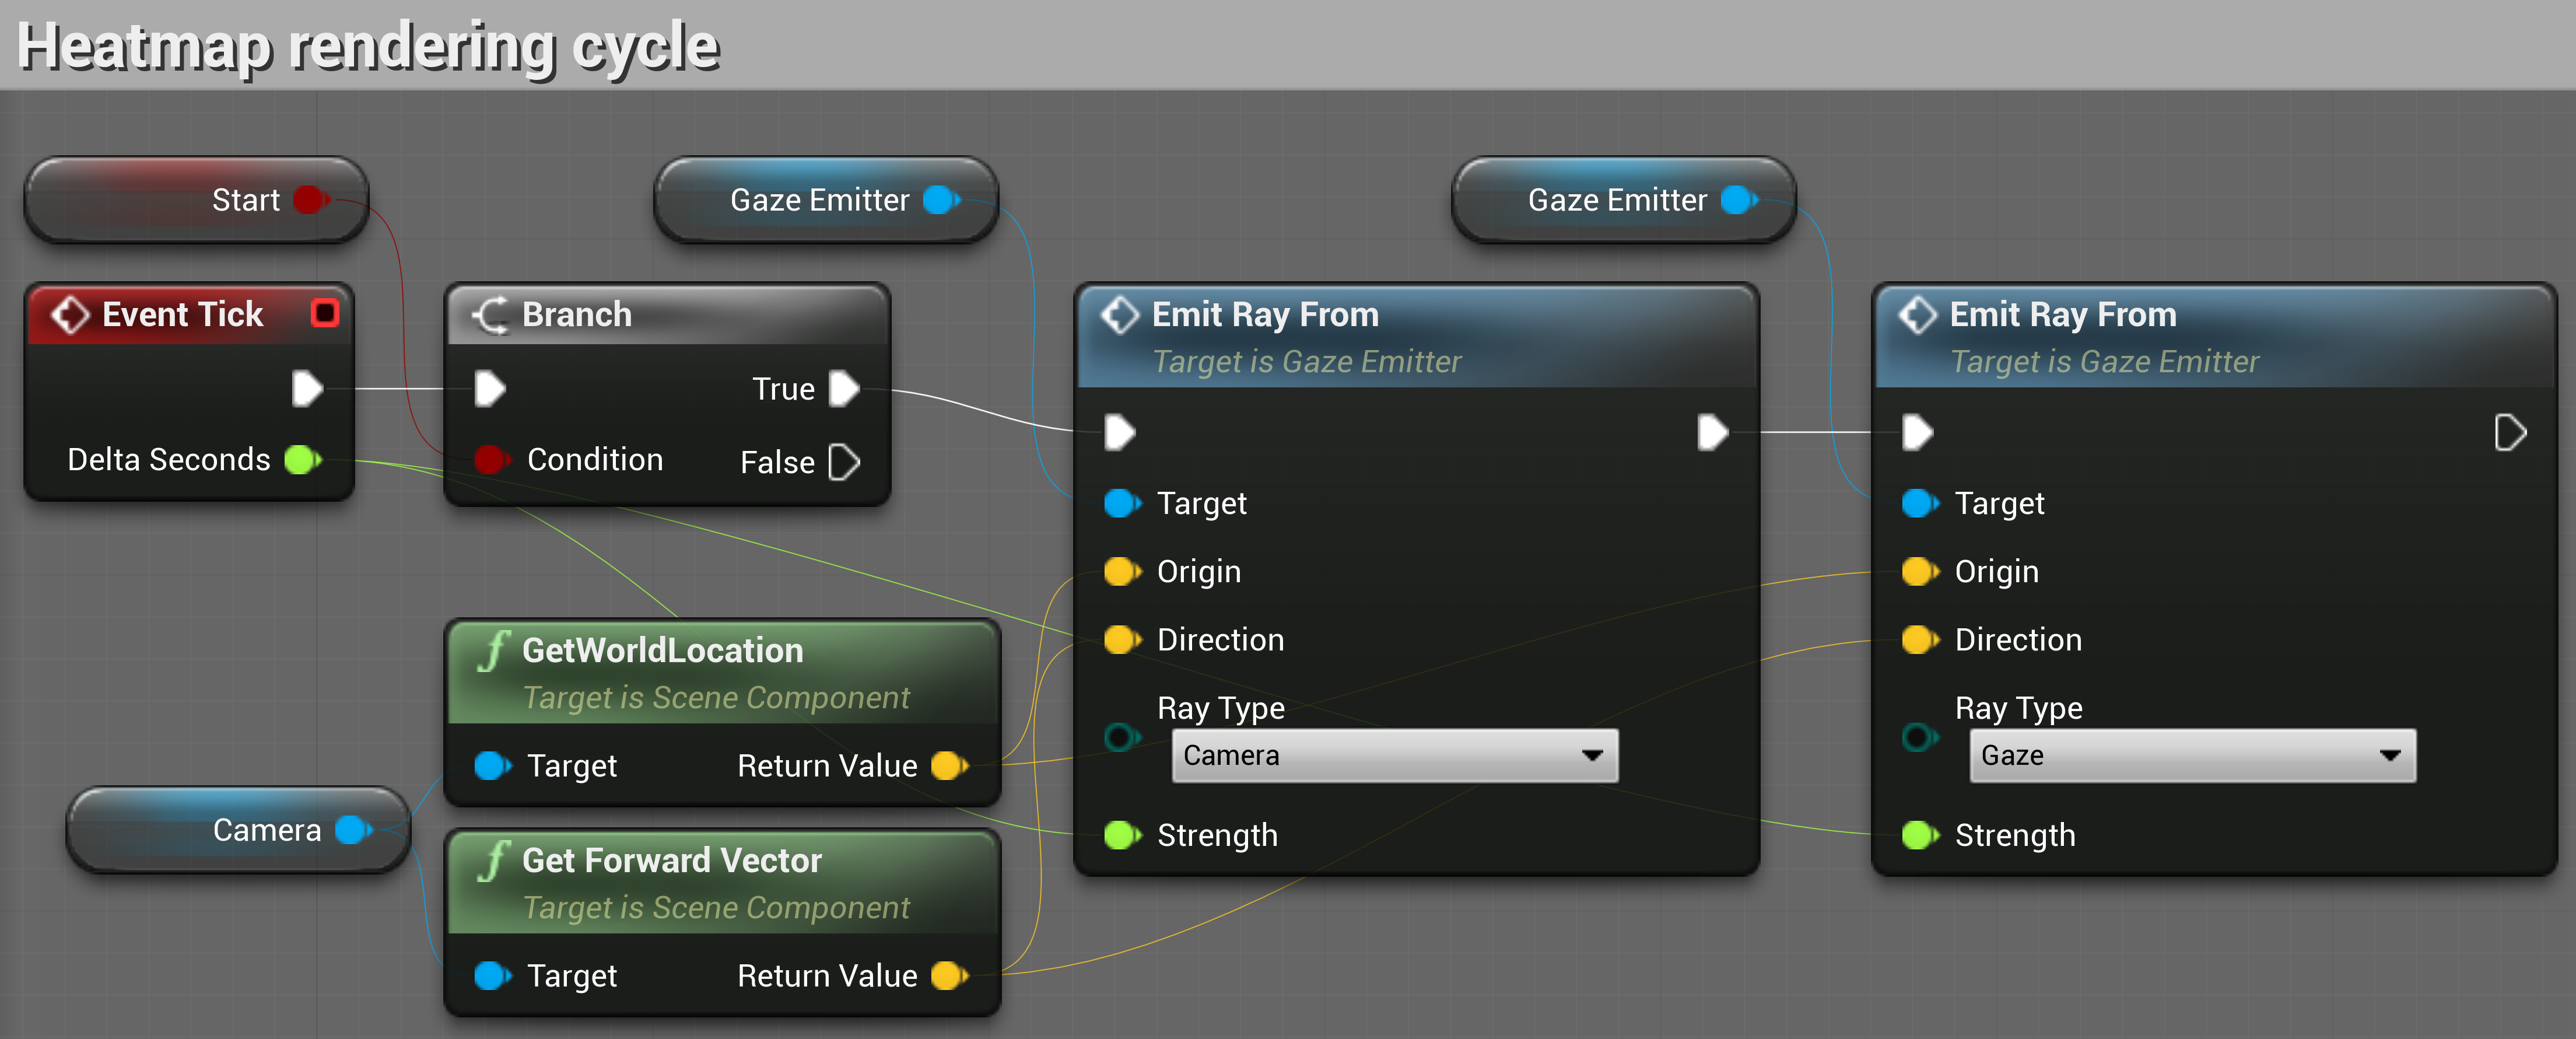
\includegraphics[width=\textwidth]{img/heatmap-rendering-cycle.png}
    \caption{VRCollector Tick Event sending rays from virtual camera.}
    \label{fig:heatmap-rendering-cycle}
\end{figure}

\pagebreak{}

\subsubsection*{SceneObserver}

This pawn allows one to view the~scene after the~heatmaps have been measured. This is a~pawn of type Character, so it contains its own collider and basic movement functionality. Unlike the~VRCollector, this is a~pawn that traverses the~scene conventionally and bumps into objects. In Figure~\ref{fig:load-heatmaps-character} its initialisation can be seen, where it specifies its height and loads all heatmaps that are stored in the~\path{C:/ProgramData/NC_ET/} directory structure. Use the~H key to switch between heatmap visualisations. There are three different options. First, the~original material without heatmaps, then the~TrailCompare from Section~\ref{sec:trail-compare-implementation} and finally the~HeatMaterial from Section~\ref{sec:heat-material-implementation}.

\begin{figure}[!ht]\centering
    \begin{subfigure}[b]{\textwidth}
        \centering
        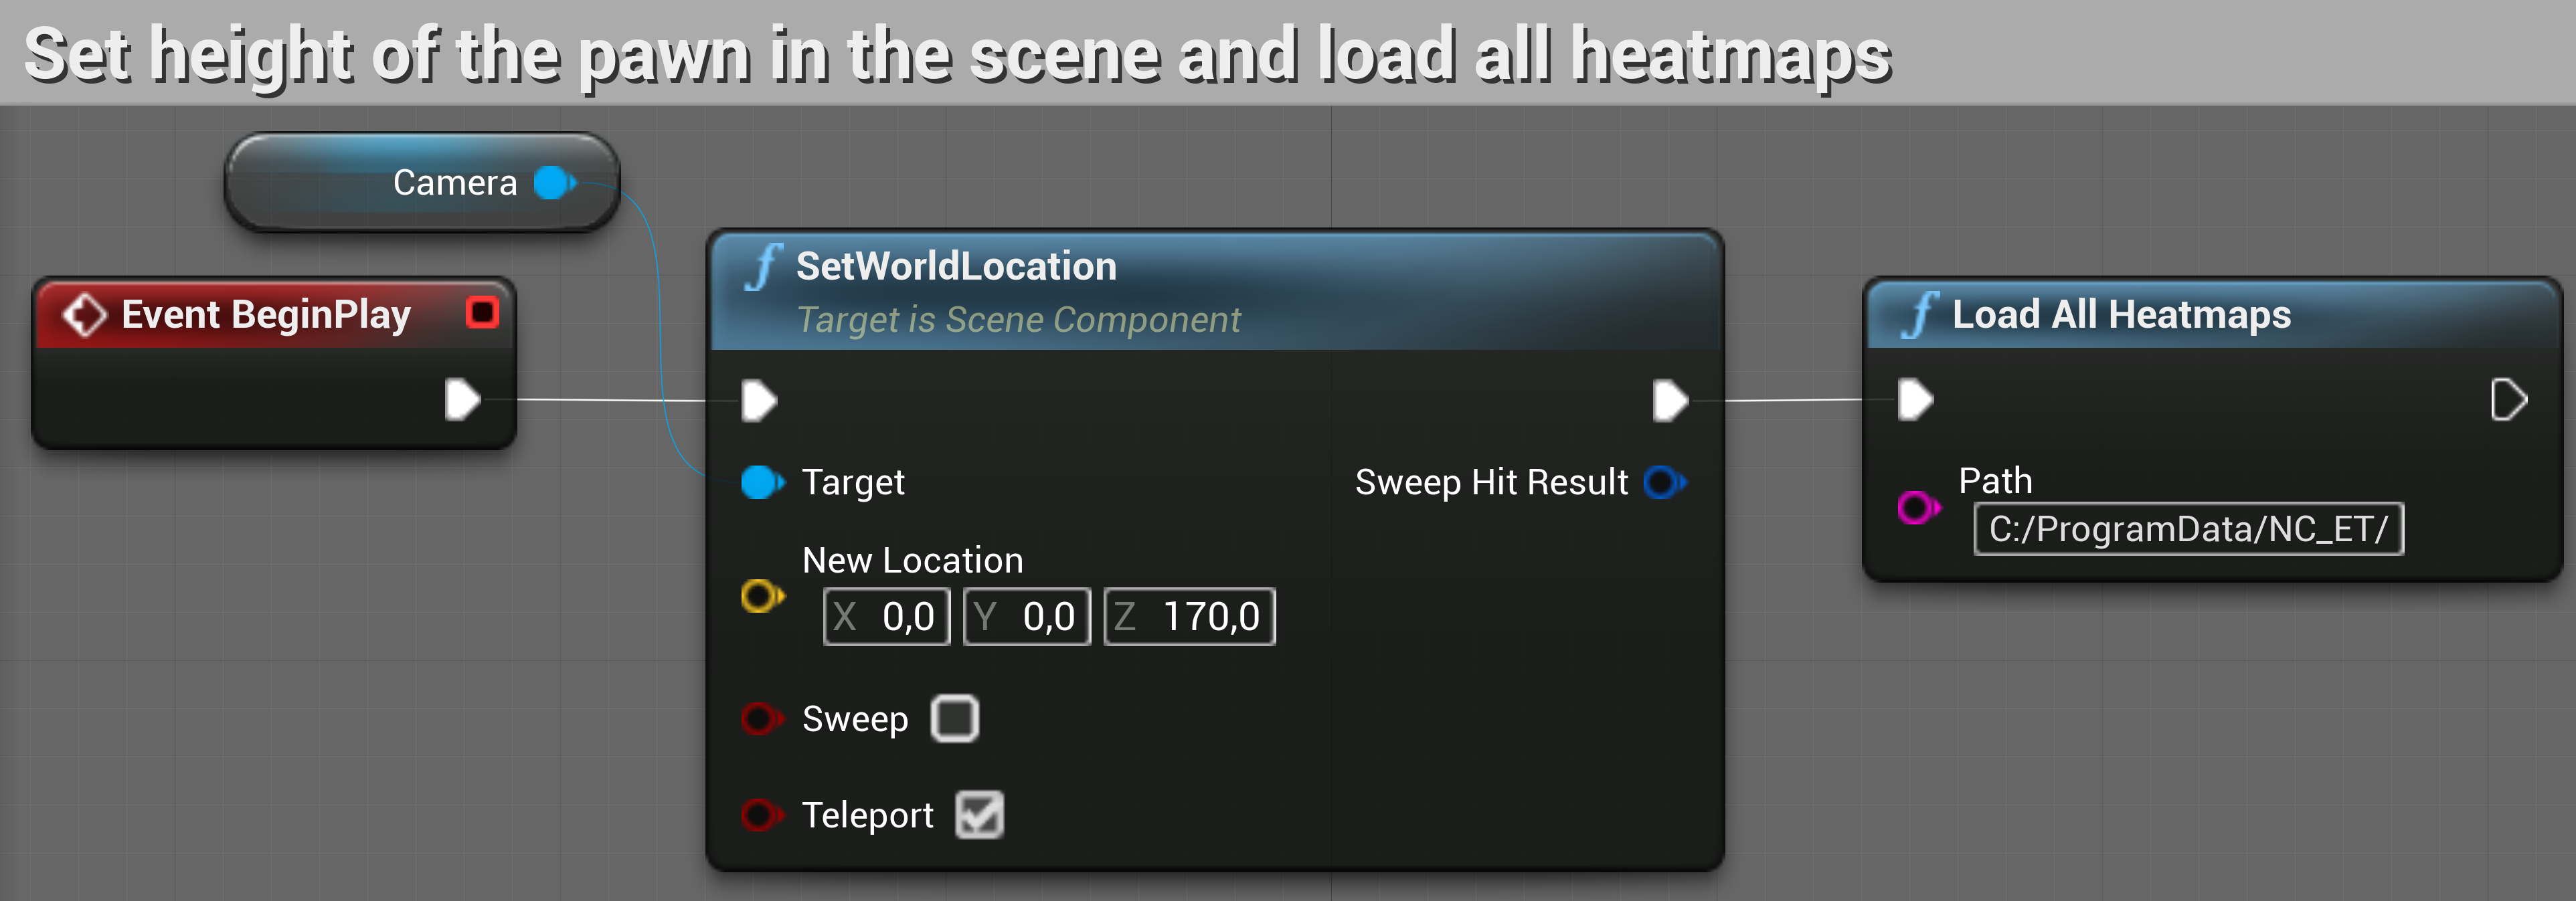
\includegraphics[width=0.8\textwidth]{img/initialise-character-pawn.png}
        \caption{Initialise character and load heatmaps.}
        \label{fig:load-heatmaps-character}
    \end{subfigure}
    \begin{subfigure}[b]{\textwidth}
        \centering
        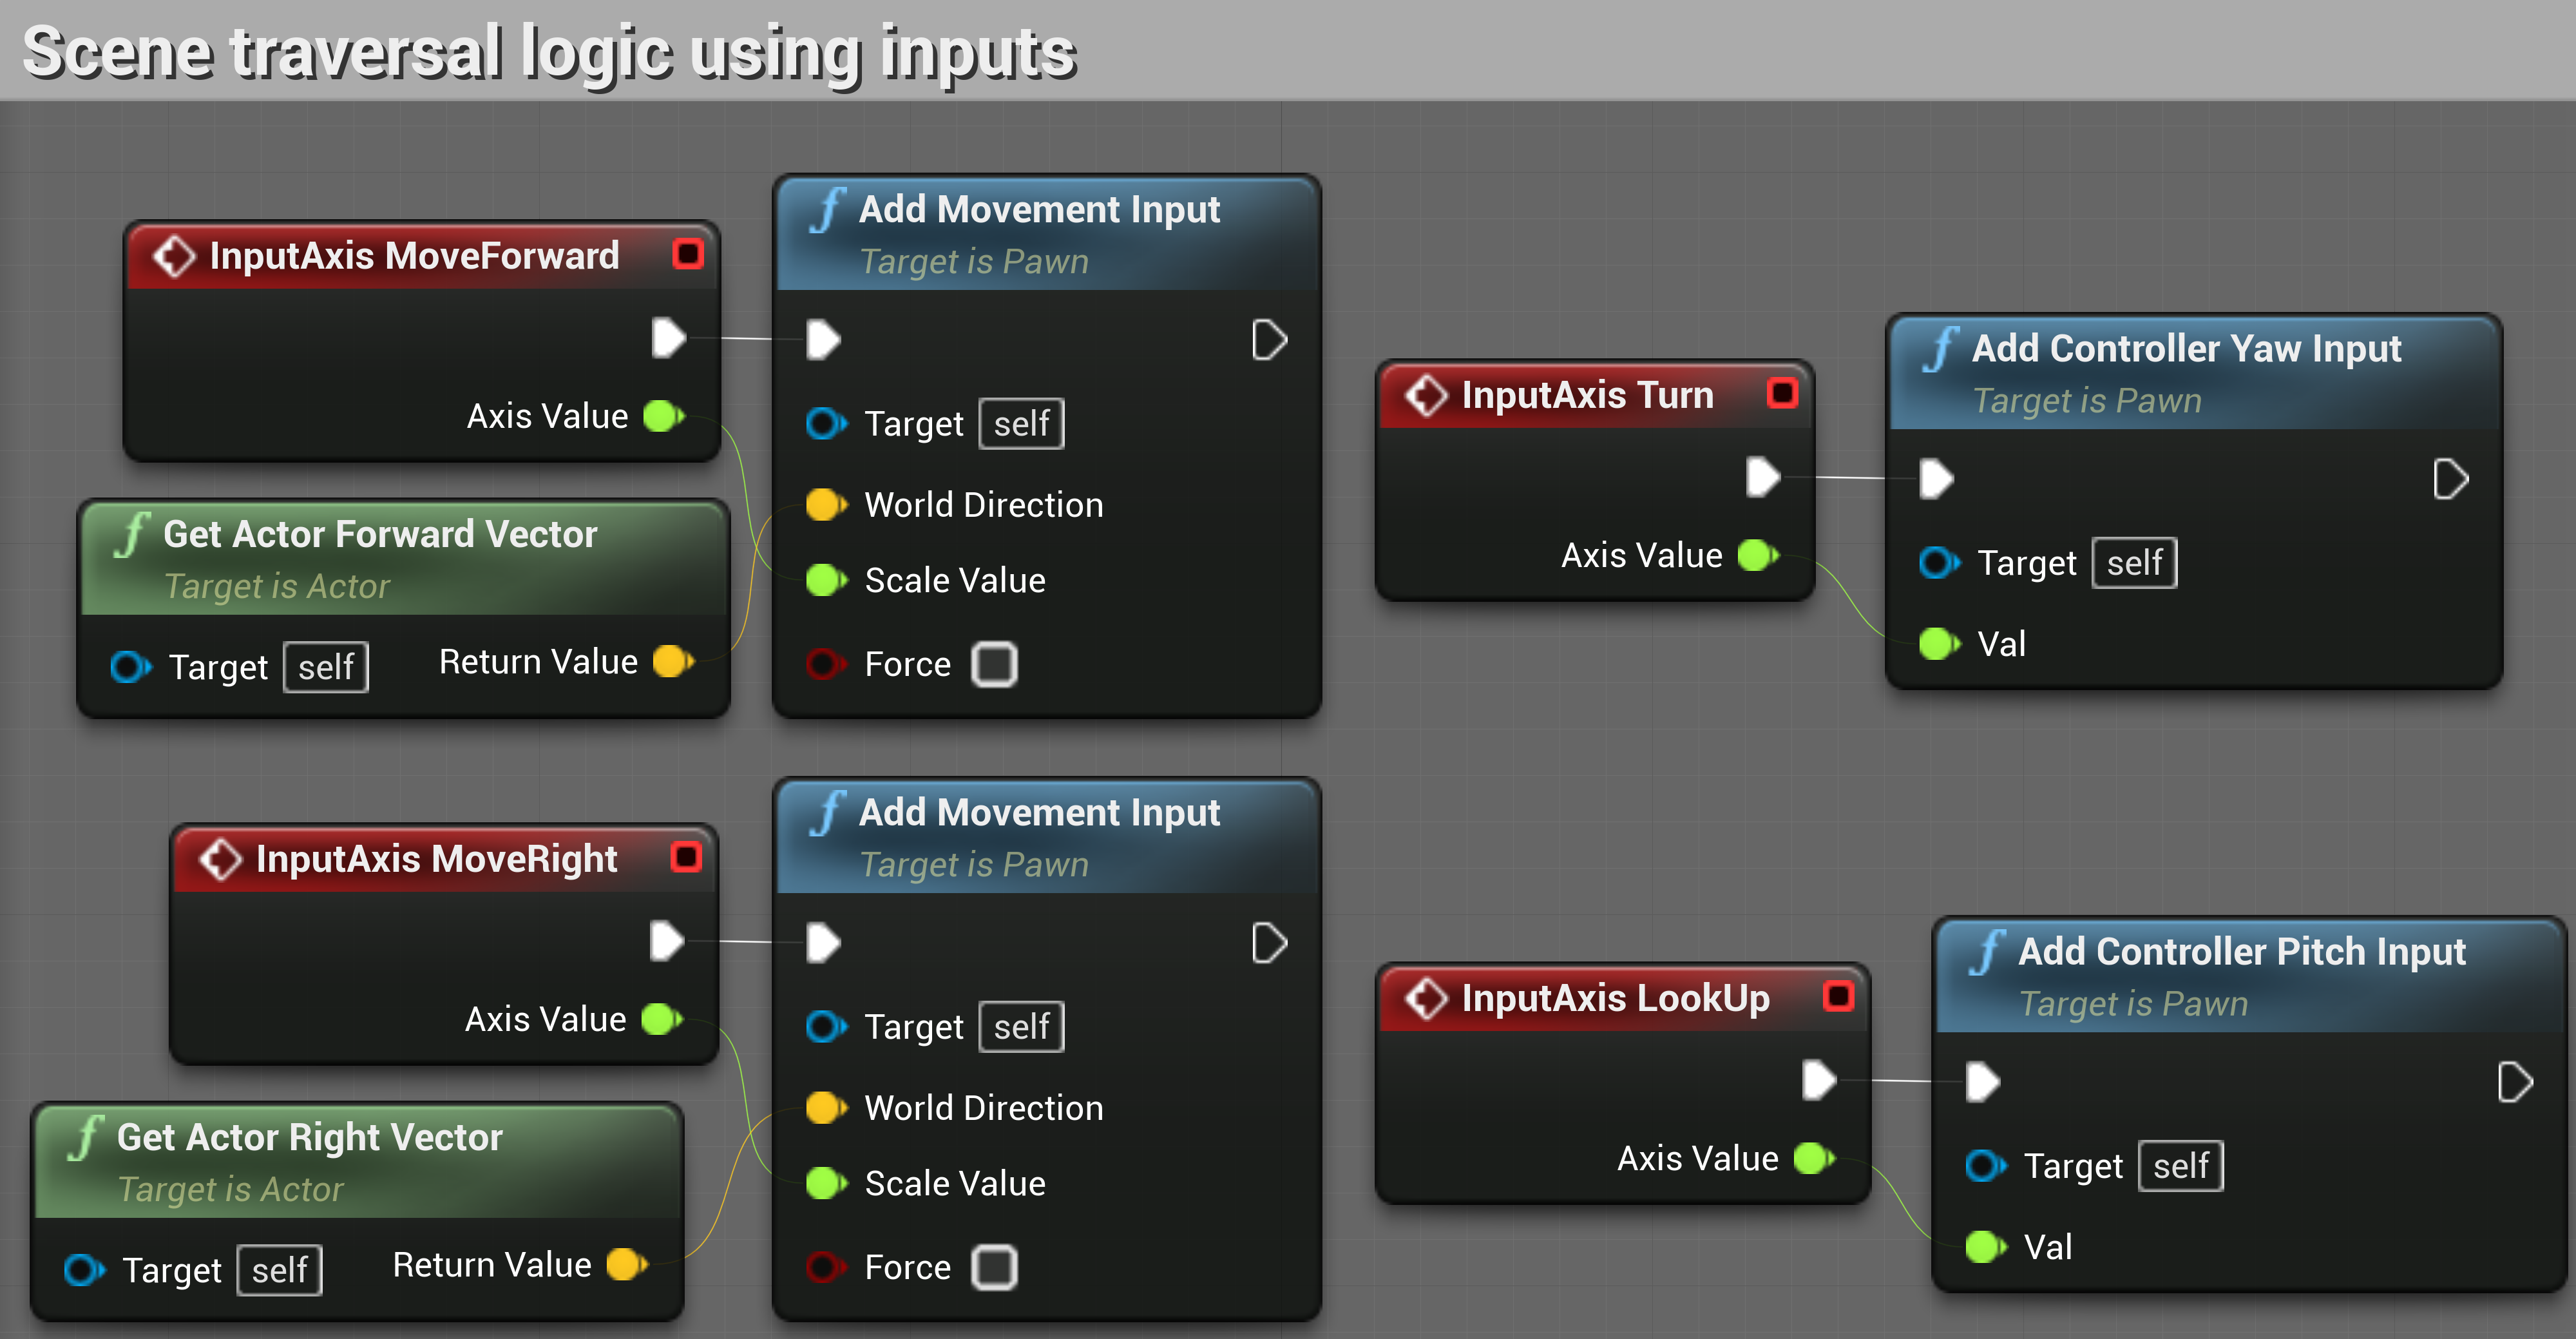
\includegraphics[width=\textwidth]{img/character-traversal.png}
        \caption{Traversal character logic.}
    \end{subfigure}
    \begin{subfigure}[b]{\textwidth}
        \centering
        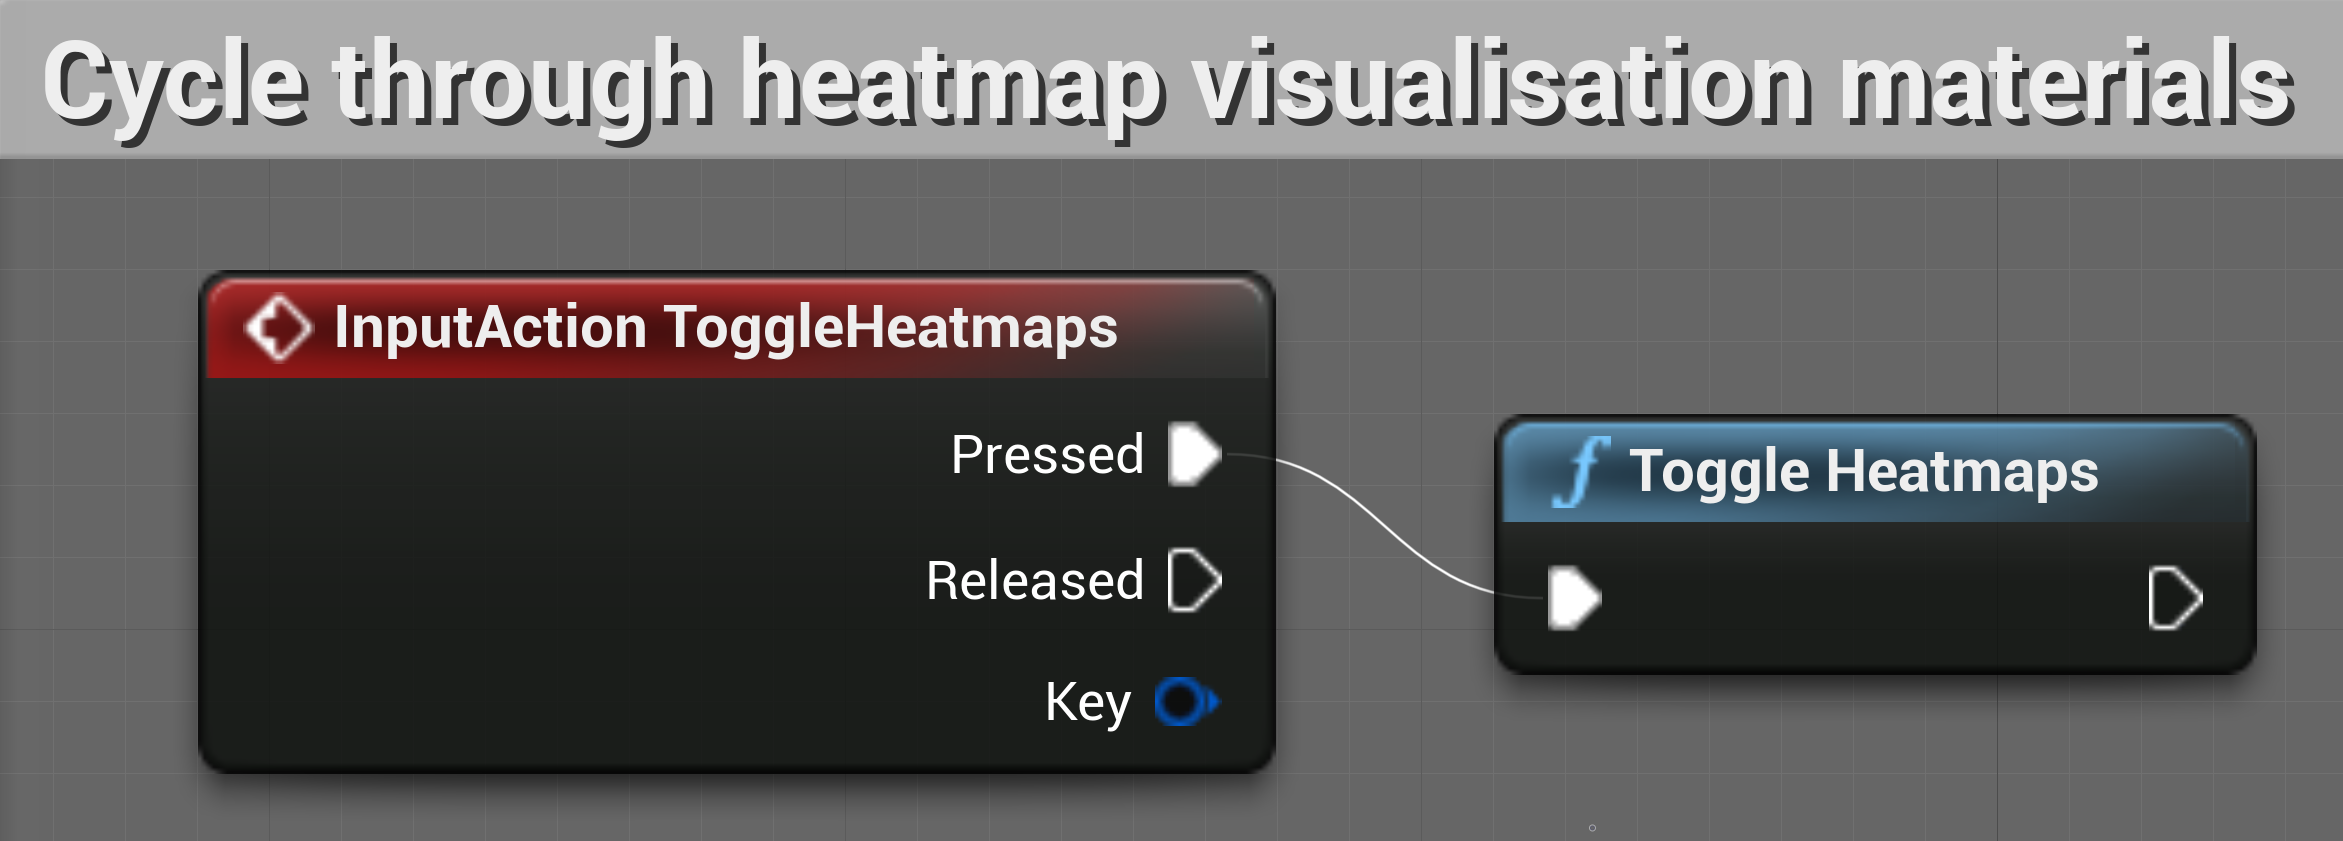
\includegraphics[width=0.6\textwidth]{img/toggle-heatmaps.png}
        \caption{Toggle heatmap visualisation.}
    \end{subfigure}
    \caption{SceneObserever Event Graph.}
    \label{fig:character-event-graph}
\end{figure}

\subsection{Controls}

Both Pawns use this simple control interface. All button mappings can be seen in Figure~\ref{fig:controls}.

\begin{figure}[!ht]\centering
    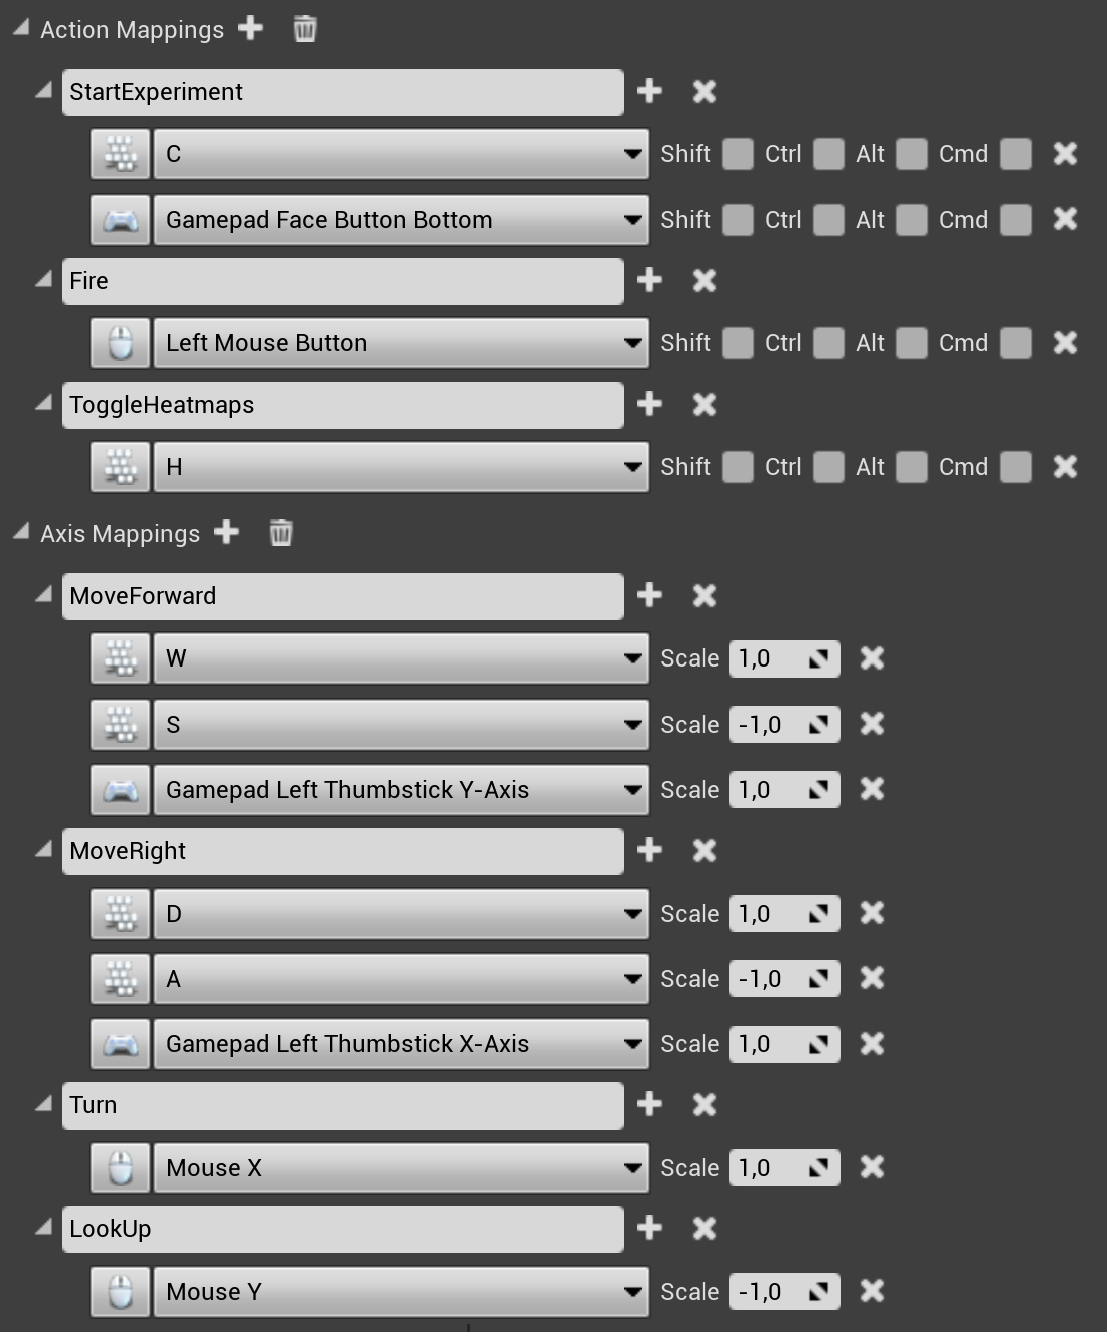
\includegraphics[width=\textwidth]{img/controls.png}
    \caption{Control scheme of the~unreal project with experiment.}
    \label{fig:controls}
\end{figure}

\pagebreak{}

\section{XTAL}

This section describes the~setup of the~XTAL headset within the~3D CAVE laboratory at the~Faculty of Mechanical Engineering of CTU. It also presents issues with the~current beta OpenXR runtime by Vrgineers~\cite{vrgineers-openxr-soft} and its unsuccessful troubleshooting. Note that the~lab has an~older generation of XTAL than the~current XTAL 3.

\subsection{Setup}
The~laboratory has set up several VICON tracking cameras that collectively acquire the~absolute position of defined objects in this space using small reflective spheres. Several of these spheres are attached to XTAL. The~VICON system obtains the~absolute position of these spheres and sends them as an~overall object defined as \emph{Xtal01} over the~network. In the~settings of the~VR Tool runtime, which is the~driver for the~XTAL headset~\cite{vr-tool}, the~positioning system can be set to VICON. There, it can specify the~IP address of the~system that sends these positioning data.

Regarding XTAL itself, Figure~\ref{fig:vr-tools-settings} shows the~eye runtime settings. Functions such as auto-IPD can be triggered, which is measured using ET to automatically adjust the~lens distance inside. There is also a~calibration section for the~ET. The~user must always run a~new calibration when a~programme is started. Advanced calibration is a~seven-point calibration that results in more precise measurements. 

\begin{figure}[!ht]\centering
    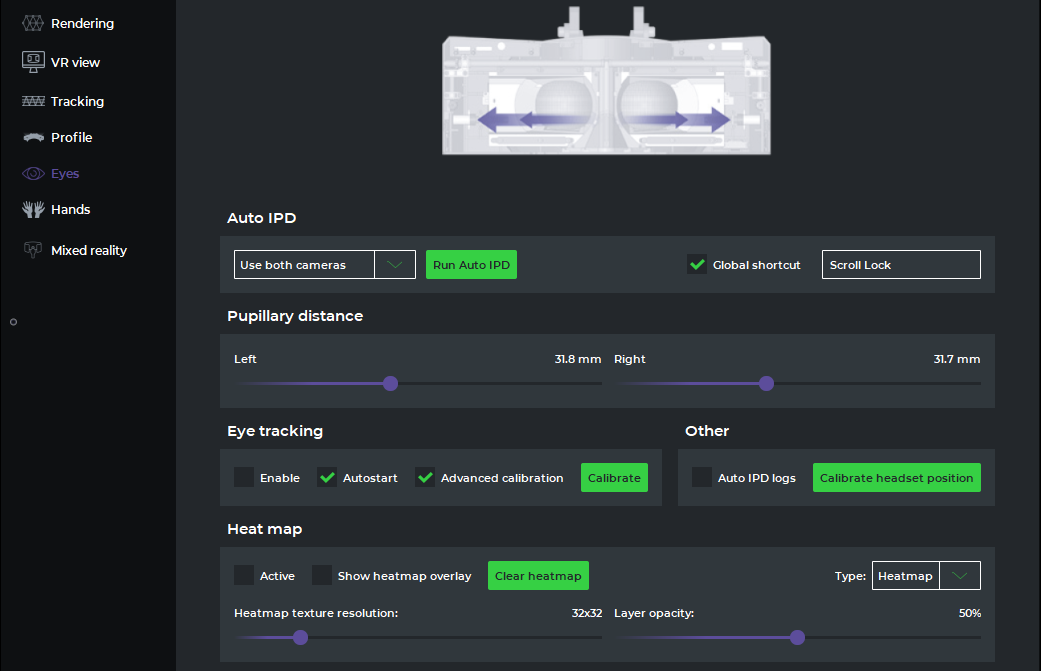
\includegraphics[width=0.9\textwidth]{img/runtime-eye-settings.png}
    \caption{Vrgineers VR Tool runtime eye settings.~\cite{vr-tool}}
    \label{fig:vr-tools-settings}
\end{figure}

\subsection{Troubleshooting}

The~main problem that occurred was the~instability of the~OpenXR XTAL runtime, which caused regular crashes of the~entire UEEditor during the~VR Preview in the~Unreal project. The~VR Preview sometimes lasted for a~full three minutes before crashing and sometimes did not even turn on. The~error message can be seen in Figure~\ref{fig:unreal-error-msg}.

\pagebreak{}
The~latest version of OpenXR runtime from Vrgineers~\cite{vrgineers-openxr-soft}, sent via email, was tested. The~runtime was still in beta at the~time of writing, and it was not possible to resolve this issue for Unreal Engine 4.27.

Support from Vrgineers was consulted on this issue, and they said that they are also experiencing runtime crashes of the~UEEditor for unknown reasons, but not at such frequent intervals~\cite{vrginners-email}. It has been tested to see if the~debugging tools used in UEEditor are to blame for this. Although the~crashes were not as sudden, the~project always lasted at least half a~minute; it did not solve the~problem.

While the~VR Preview was running, it was possible to calibrate the~ET and send rays out into the~scene. The~problem is that this process is rather long, and before the~participant could get to the~measuring part, the~whole programme would crash. It was tested to see if it would crash even when running the~standalone version of the~game. In this case, it was not determined whether this would solve the~problem because the~OpenXR runtime does not initialise the~XTAL headset to display the~scene inside, even though the~Start in VR option is enabled in the~project settings. The~console command ''\emph{stereo on}`` for the~Blueprint node \emph{Execute Console Command} was also tried, but nothing changed. It will run only for the~VR Preview in the~UEEditor.

The~Vrgineers support recommended migrating the~entire project to Unreal Engine 5, as it contains a~much more stable implementation of OpenXR communication. This was unsuccessful; details can be seen in the~Appendix~\ref{appendix:UE5}.

It was decided, after consultation with the~thesis supervisor, to use the~Vrgineers stable SDK plugin for Unreal Engine~\cite{vrgineers-unreal-sdk}, which includes the~original native runtime. However, this does not allow the~use of ET.

\begin{figure}[!t]\centering
    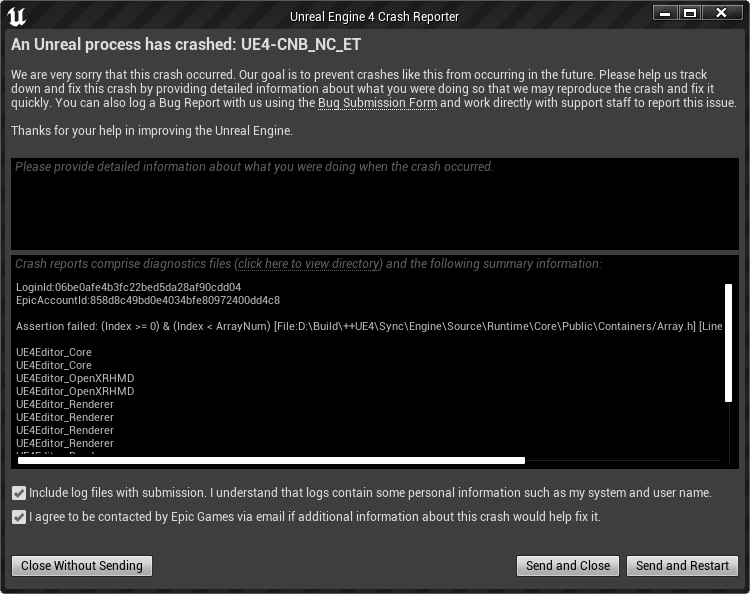
\includegraphics[width=0.95\textwidth]{img/unreal-error-msg.png}
    \caption{UEEditor crash log after OpenXR VR Preview.}
    \label{fig:unreal-error-msg}
\end{figure}

\pagebreak{}

\section{Data collecion}
\label{sec:data-collection}

Due to the~instability of the~OpenXR runtime, the~originally intended eye tracking experiment could not be performed, so it was decided that the~data would only be collected using a~forward vector camera in a~virtual scene in which the~participant would walk around using the~XTAL headset. 

The~plug-in created in this thesis, Chapter~\ref{chap:implementation}, contains raycasting functionality that can be easily used in any Unreal project. Thus, it already depends only on using a~working VR headset with ET. It has been tested on an~unstable XTAL runtime that the~feature works and sends rays into the~scene. It was not possible to use any other headset as an~alternative due to the~unavailability of other headsets and the~lack of time to incorporate the~changes into the~thesis.

The~test experiment will be carried out as originally intended, but without the~use of ET. It will collect both Gaze and Camera heatmaps, although it will only emit rays from the~forward vector of the~camera. This will serve as a~demonstration of what it would look like if working ET hardware was used.

\subsection{Test scenario}

The~test scenario used in this experiment is a~scene traversal by a~person who has not previously seen it. Each participant creates their own collection of heatmaps. These heatmaps will be used to determine which object most interested the~group of participants or where the~most textures intersected their trails.

\subsection{Measurement process}

One measurement consisted of first placing a~headset on the~participant to set their PID. Then, the~Unreal Engine project was launched with the~VRCollector pawn, defined in Section~\ref{sec:pawns}. The~XTAL in the~lab is connected to the~computer, which is used as a~backpack, to walk around the~lab. The~computational part of the~backpack had to be unplugged from the~charging dock and attached to its other part. The~backpack was put on by the~participant with the~headset. Before this, the~participant was instructed how to move around the~scene using a~game controller. They could have moved around without a~controller, but they would soon have hit a~wall in the~lab because the~exhibition is much bigger, so a~controller was necessary. The~speed of movement resembled a~fast walk. They were also informed that the~scene was an~exhibit of the~Czech National Bank. After ensuring that the~participant was ready, a~test period of three minutes was started. During this time, the~participant was free to walk around the~scene as they wished. A~participant was looking at the~scene that was with its original materials. Heatmaps were produced in the~background. At the~end of the~three minutes, all heatmaps were saved in the~\path{C:/ProgramData/NC_ET/} path and the~programme was stopped.

Videos of the~measurements were recorded. Participants 4 and 8 were chosen to demonstrate the~experiment. Their recorded session is in the~enclosed media in the~\path{video} folder. All heatmaps from all participants are compressed in the~\path{experiment/data/ParticipantData.zip} file.


\section{Resultant data}

A~total of 12 measurements were made, so 12 different heatmap collections were produced. These data were grouped into the~DATA folder and each measurement was in the~folder of a~numbered participant. Each participant contains a~Camera and Gaze folder, due to the~two different types of heatmap. The~Python merger script from Section~\ref{sec:python} was put in the~same folder, which merged these participants into folder \path{ResultantData}. The~same folder is in the~enclosed media in the~\path{data} folder.

There are several information panels in the~exhibition scene. The~resultant data showed that they were the~majority target of interest. It is possible to turn on the~Unreal Project and view the~data by running the~scene with the~SceneObserver pawn. The~data folder structure, along with the~Gaze and Camera folders, should be put in the~\path{C:/ProgramData/NC_ET/} folder to view them. The~scene traversal with the~resultant data can also be viewed in \path{video/05-resultant-data-showcase.mp4}.

From the~resultant data, the~four panels that showed the~highest trail densities were selected.

\subsubsection*{Panel11}
In Figure~\ref{fig:Panel11-object-heatmaps.} it is possible to see the~difference in the~textures collected of the~\emph{Panel11} scene object.
Panel11 has the~highest intensity of its trails of all the~objects in the~scene, as shown in Figure~\ref{fig:panel11-heatmap}. The~density, on the~other hand, is not large and it can be seen that large brushes were used to produce it. This means that the~participants were looking at the~object from a~longer distance. Particularly at the~beginning of the~scene while looking around to the~left or right, this is one of the~first objects visible in the~scene. 
Five participants did not even see the~object. Only three examined it. Participant 7 is an~outlier who looked at the~object for much longer and contributed greatly to the~result. 

\subsubsection*{Panel14}
Panel14 in Figure~\ref{fig:Panel14-object-heatmaps} shows the~different variations of the~heatmaps collected from the~participants and immediately Figure~\ref{fig:Panel14-resultant-heatmaps.} shows the~resulting texture and its comparison with the~original material. Only three participants have not seen this object. Unlike Panel11, this time the~object was not only viewed from a~distance, but also seen from up close by five participants. Since it has much higher density of different twisting trails.

\subsubsection*{Panel17}
Like the~previous cases, the~results are illustrated in Figures~\ref{fig:Panel17-object-heatmaps.}~and~\ref{fig:Panel17-resultant-heatmaps.}. This is the~same case as the~Panel14. It was examined up close. Compared to the~rest, it shows in its trails that more participants noticed the~mascot of the~Czech National Bank. It is the~only object that has this part of its panel highlighted together with Panel1.

\subsubsection*{Panel2}
The~panel with the~highest trail density on its surface was Panel2, which has the~advantage of being two-sided; it has graphics on both of its sides. It is located right among the~first objects in the~whole scene, next to the~large CNB logo. Figures~\ref{fig:Panel2-object-heatmaps.} and \ref{fig:Panel2-resultant-heatmaps.}.

\newpage{}

\begin{figure}[!ht]\centering
    \begin{subfigure}[b]{0.24\textwidth}
        \centering
        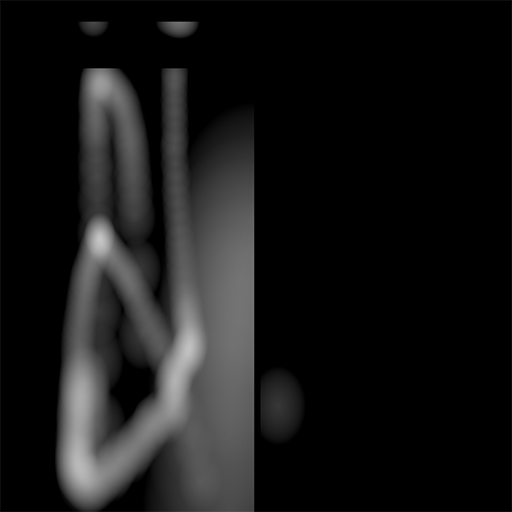
\includegraphics[width=\textwidth]{img/data/Panel11/single/1.png}
        \caption{Participant 1.}
    \end{subfigure}
    \hfill
    \begin{subfigure}[b]{0.24\textwidth}
        \centering
        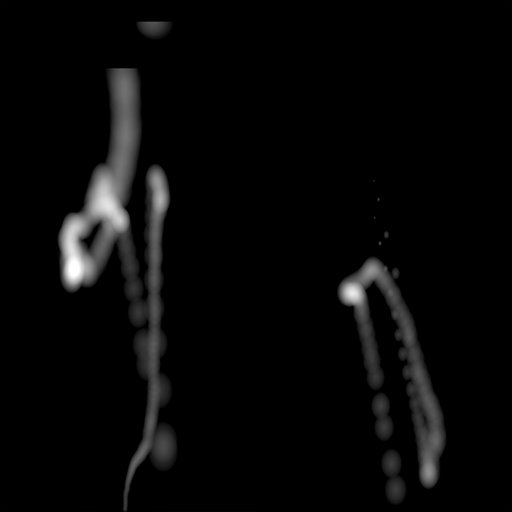
\includegraphics[width=\textwidth]{img/data/Panel11/single/2.png}
        \caption{Participant 2.}
    \end{subfigure}
    \hfill
    \begin{subfigure}[b]{0.24\textwidth}
        \centering
        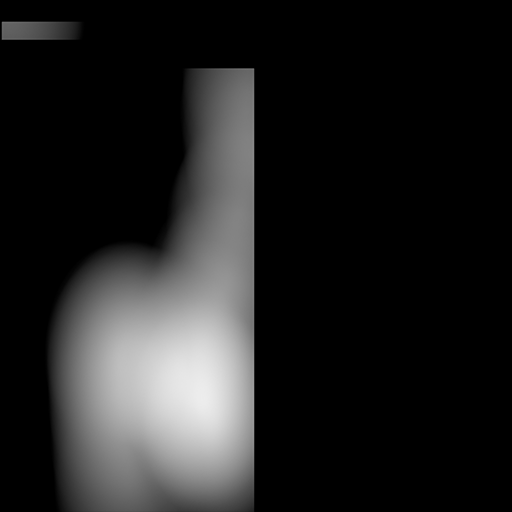
\includegraphics[width=\textwidth]{img/data/Panel11/single/3.png}
        \caption{Participant 3.}
    \end{subfigure}
    \hfill
    \begin{subfigure}[b]{0.24\textwidth}
        \centering
        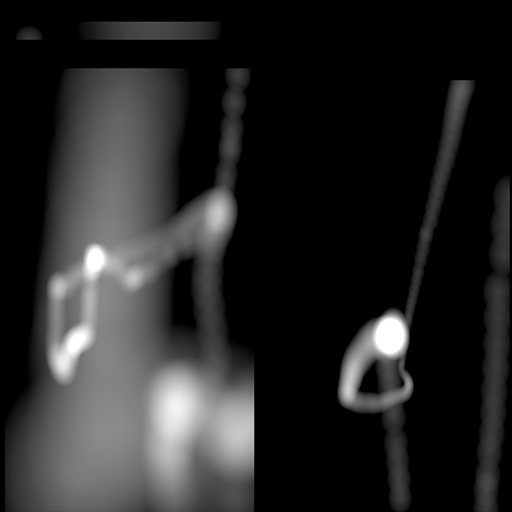
\includegraphics[width=\textwidth]{img/data/Panel11/single/4.png}
        \caption{Participant 4.}
    \end{subfigure}
    \hfill
    \begin{subfigure}[b]{0.24\textwidth}
        \centering
        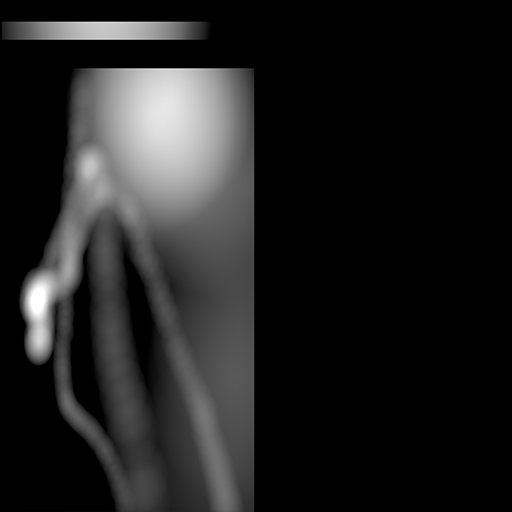
\includegraphics[width=\textwidth]{img/data/Panel11/single/5.png}
        \caption{Participant 5.}
    \end{subfigure}
    \hfill    
    \begin{subfigure}[b]{0.24\textwidth}
        \centering
        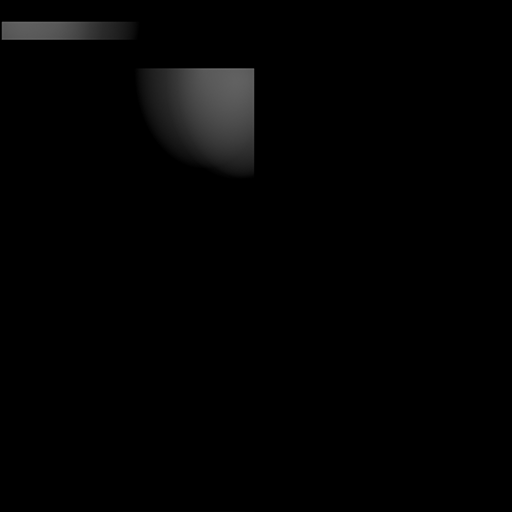
\includegraphics[width=\textwidth]{img/data/Panel11/single/6.png}
        \caption{Participant 6.}
    \end{subfigure}
    \hfill    
    \begin{subfigure}[b]{0.24\textwidth}
        \centering
        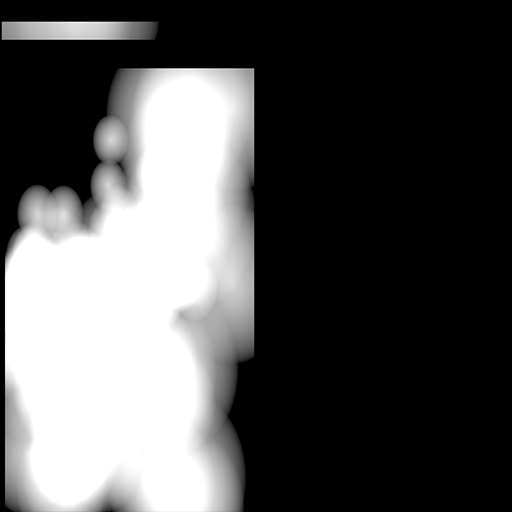
\includegraphics[width=\textwidth]{img/data/Panel11/single/7.png}
        \caption{Participant 7.}
    \end{subfigure}
    \hfill    
    \begin{subfigure}[b]{0.24\textwidth}
        \centering
        
\includegraphics[width=\textwidth]{img/data/Panel11/single/8.png}
        \caption{Participant 8.}
    \end{subfigure}
    \hfill    
    \begin{subfigure}[b]{0.24\textwidth}
        \centering
        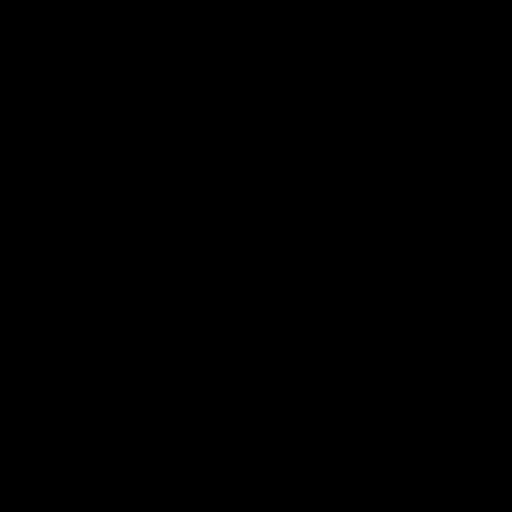
\includegraphics[width=\textwidth]{img/data/Panel11/single/9.png}
        \caption{Participant 9.}
    \end{subfigure}
    \hfill    
    \begin{subfigure}[b]{0.24\textwidth}
        \centering
        \includegraphics[width=\textwidth]{img/data/Panel11/single/10.png}
        \caption{Participant 10.}
    \end{subfigure}
    \hfill    
    \begin{subfigure}[b]{0.24\textwidth}
        \centering
        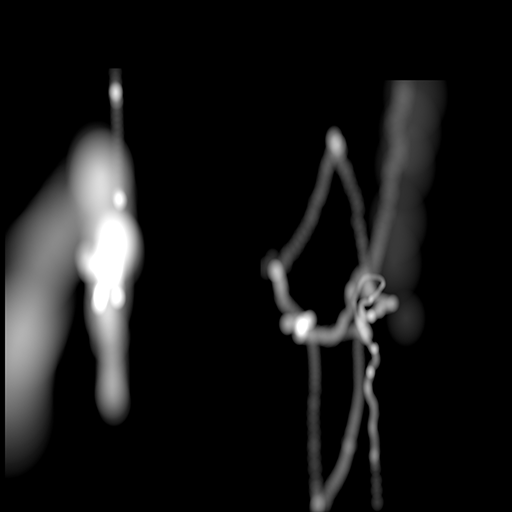
\includegraphics[width=\textwidth]{img/data/Panel11/single/11.png}
        \caption{Participant 11.}
    \end{subfigure}
    \hfill    
    \begin{subfigure}[b]{0.24\textwidth}
        \centering
        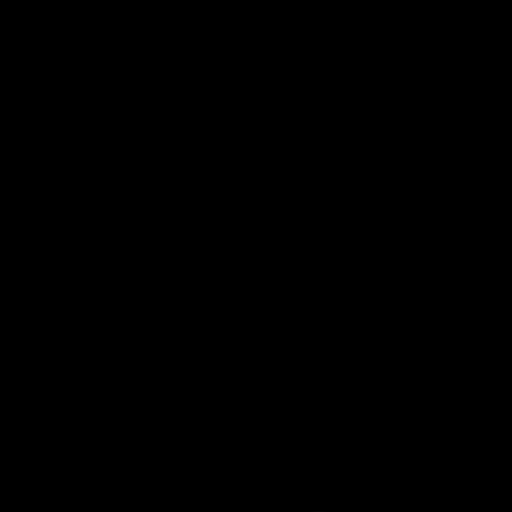
\includegraphics[width=\textwidth]{img/data/Panel11/single/12.png}
        \caption{Participant 12.}
    \end{subfigure}
    \caption{Heatmap texture variants of Panel11 object.}
    \label{fig:Panel11-object-heatmaps.}
\end{figure}


\begin{figure}[!ht]\centering
    \begin{subfigure}[b]{0.31\textwidth}
        \centering
        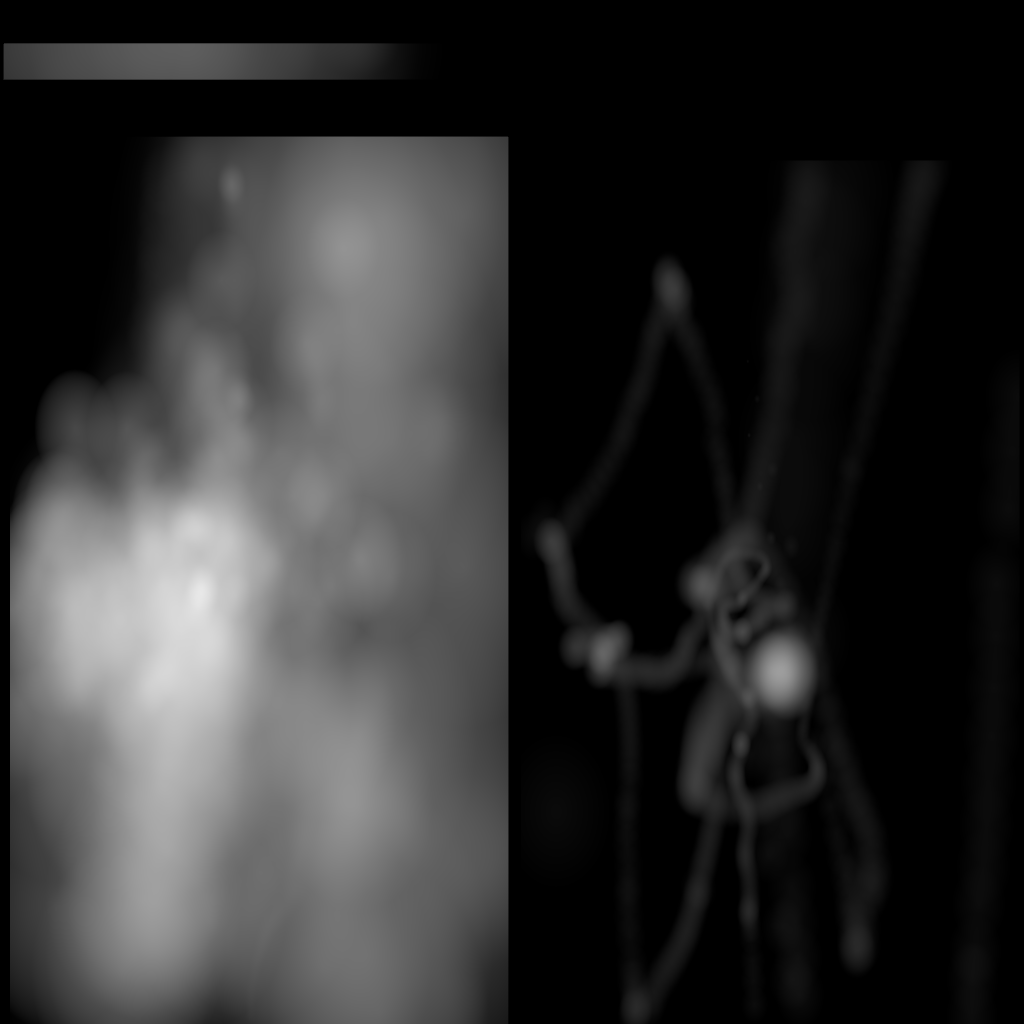
\includegraphics[width=\textwidth]{img/data/Panel11/resultant/Result.png}
        \caption{Result gaze heatmap texture.}
    \end{subfigure}
    \hfill
    \begin{subfigure}[b]{0.335\textwidth}
        \centering
        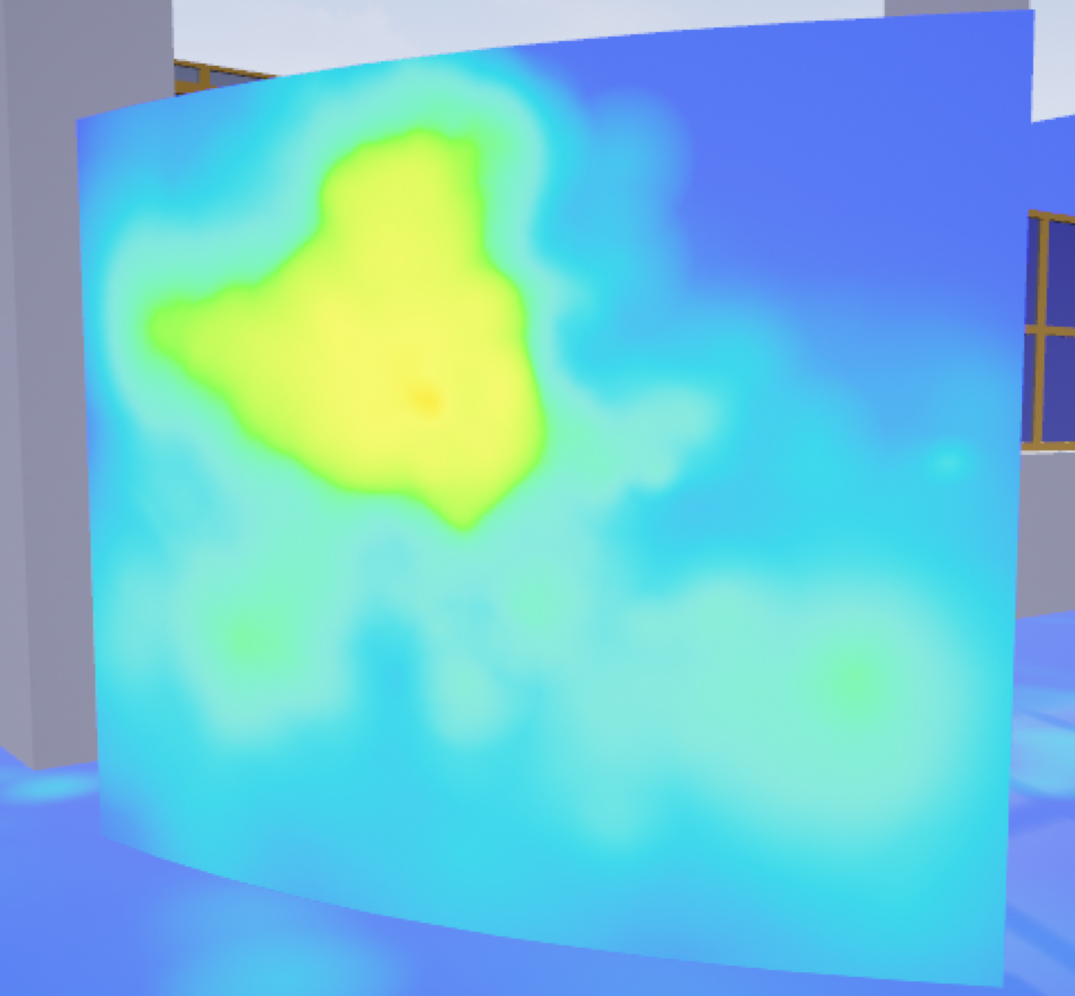
\includegraphics[width=\textwidth]{img/data/Panel11/resultant/heatmap.png}
        \caption{Result gaze heatmap on object.}
        \label{fig:panel11-heatmap}
    \end{subfigure}
    \hfill
    \begin{subfigure}[b]{0.33\textwidth}
        \centering
        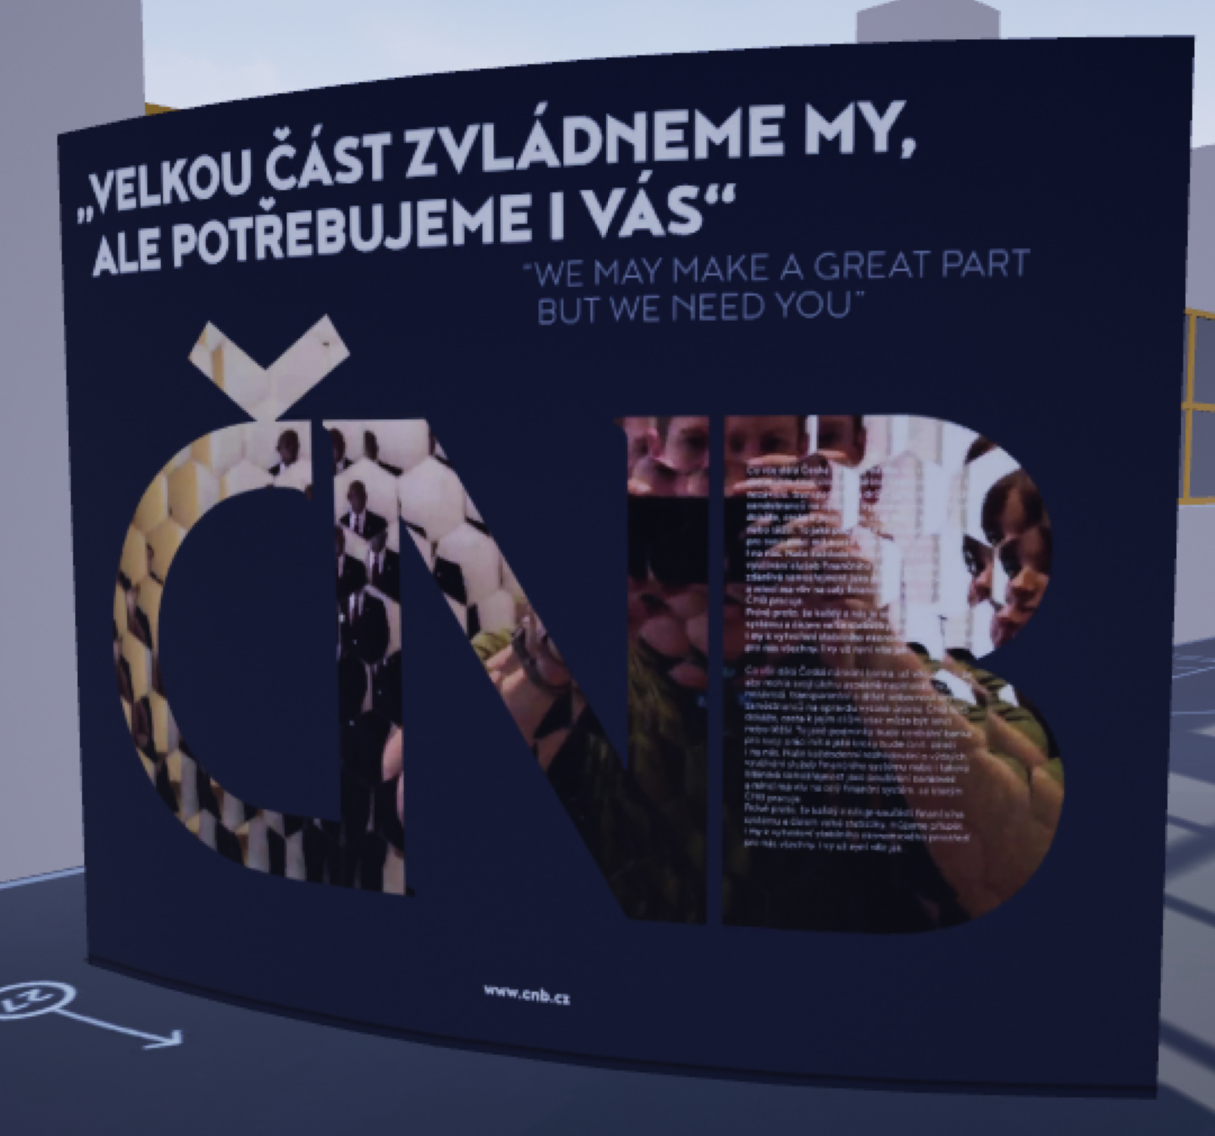
\includegraphics[width=\textwidth]{img/data/Panel11/resultant/original.png}
        \caption{Panel11 original material.}
    \end{subfigure}
    \caption{Resultant heatmap of Panel11.}
    \label{fig:Panel11-resultant-heatmaps.}
\end{figure}


\begin{figure}[!ht]\centering
    \begin{subfigure}[b]{0.24\textwidth}
        \centering
        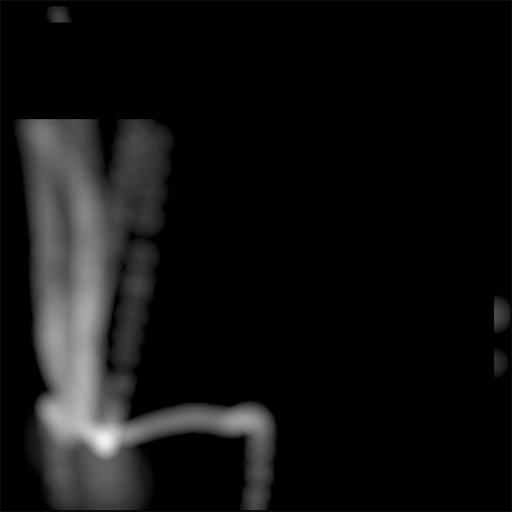
\includegraphics[width=\textwidth]{img/data/Panel14/single/1.png}
        \caption{Participant 1.}
    \end{subfigure}
    \hfill
    \begin{subfigure}[b]{0.24\textwidth}
        \centering
        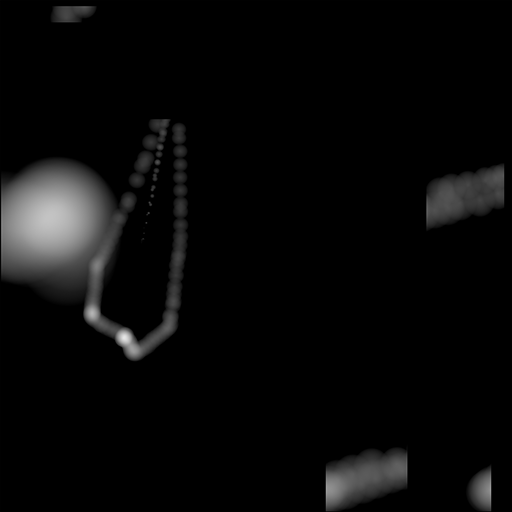
\includegraphics[width=\textwidth]{img/data/Panel14/single/2.png}
        \caption{Participant 2.}
    \end{subfigure}
    \hfill
    \begin{subfigure}[b]{0.24\textwidth}
        \centering
        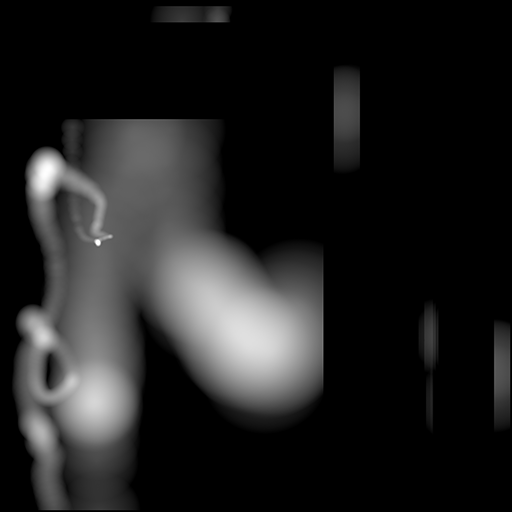
\includegraphics[width=\textwidth]{img/data/Panel14/single/3.png}
        \caption{Participant 3.}
    \end{subfigure}
    \hfill
    \begin{subfigure}[b]{0.24\textwidth}
        \centering
        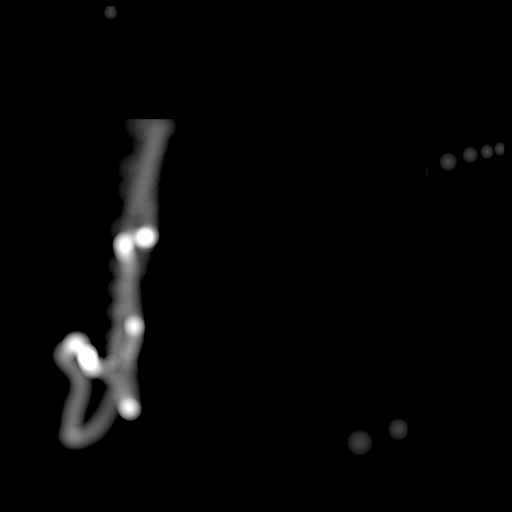
\includegraphics[width=\textwidth]{img/data/Panel14/single/4.png}
        \caption{Participant 4.}
    \end{subfigure}
    \hfill
    \begin{subfigure}[b]{0.24\textwidth}
        \centering
        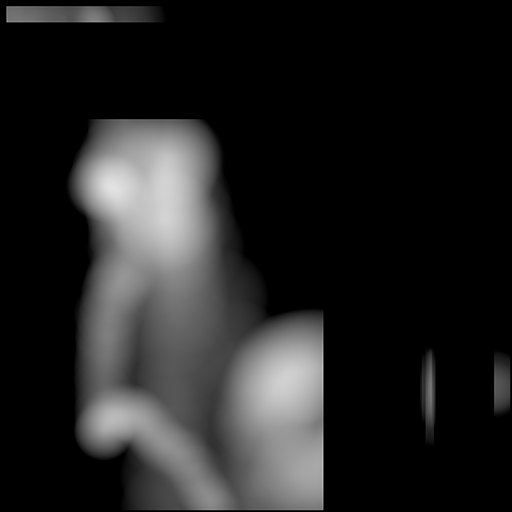
\includegraphics[width=\textwidth]{img/data/Panel14/single/5.png}
        \caption{Participant 5.}
    \end{subfigure}
    \hfill    
    \begin{subfigure}[b]{0.24\textwidth}
        \centering
        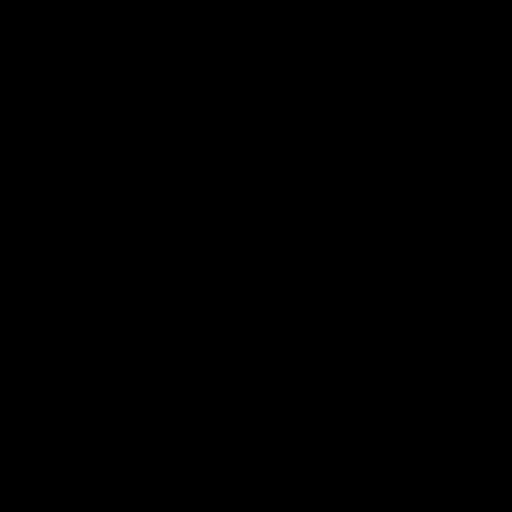
\includegraphics[width=\textwidth]{img/data/Panel14/single/6.png}
        \caption{Participant 6.}
    \end{subfigure}
    \hfill    
    \begin{subfigure}[b]{0.24\textwidth}
        \centering
        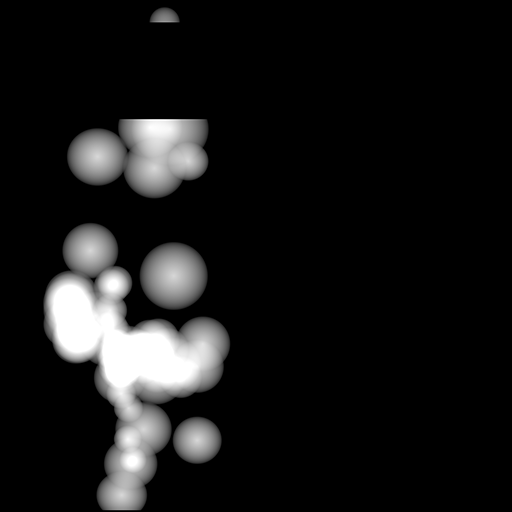
\includegraphics[width=\textwidth]{img/data/Panel14/single/7.png}
        \caption{Participant 7.}
    \end{subfigure}
    \hfill    
    \begin{subfigure}[b]{0.24\textwidth}
        \centering
        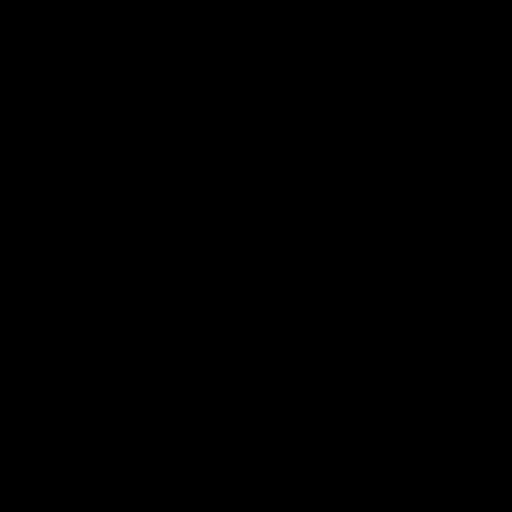
\includegraphics[width=\textwidth]{img/data/Panel14/single/8.png}
        \caption{Participant 8.}
    \end{subfigure}
    \hfill    
    \begin{subfigure}[b]{0.24\textwidth}
        \centering
        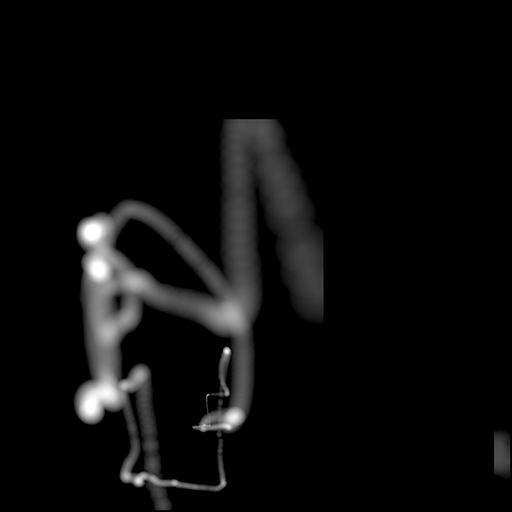
\includegraphics[width=\textwidth]{img/data/Panel14/single/9.png}
        \caption{Participant 9.}
    \end{subfigure}
    \hfill    
    \begin{subfigure}[b]{0.24\textwidth}
        \centering
        \includegraphics[width=\textwidth]{img/data/Panel14/single/10.png}
        \caption{Participant 10.}
    \end{subfigure}
    \hfill    
    \begin{subfigure}[b]{0.24\textwidth}
        \centering
        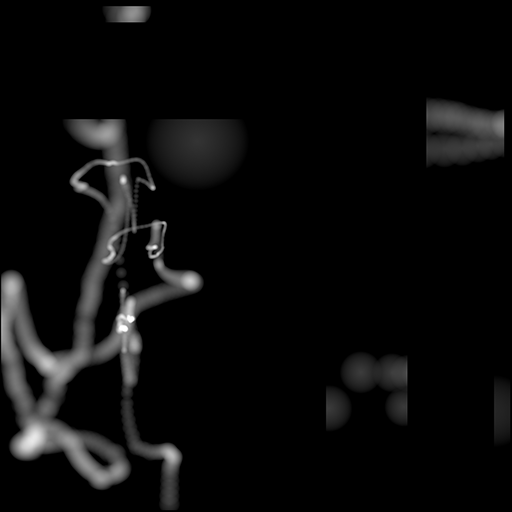
\includegraphics[width=\textwidth]{img/data/Panel14/single/11.png}
        \caption{Participant 11.}
    \end{subfigure}
    \hfill    
    \begin{subfigure}[b]{0.24\textwidth}
        \centering
        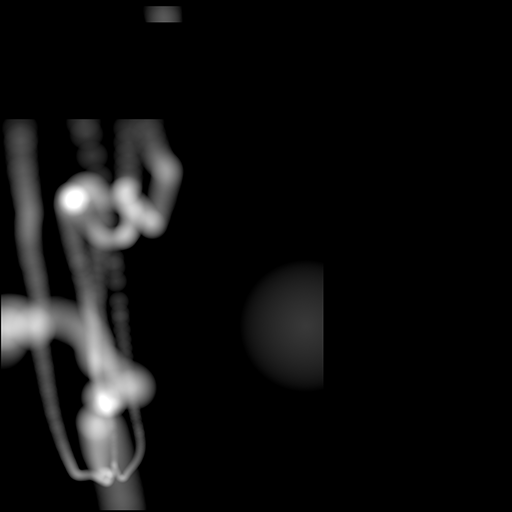
\includegraphics[width=\textwidth]{img/data/Panel14/single/12.png}
        \caption{Participant 12.}
    \end{subfigure}
    \caption{Heatmap texture variants of Panel14 object.}
    \label{fig:Panel14-object-heatmaps}
\end{figure}


\begin{figure}[!ht]\centering
    \begin{subfigure}[b]{0.32\textwidth}
        \centering
        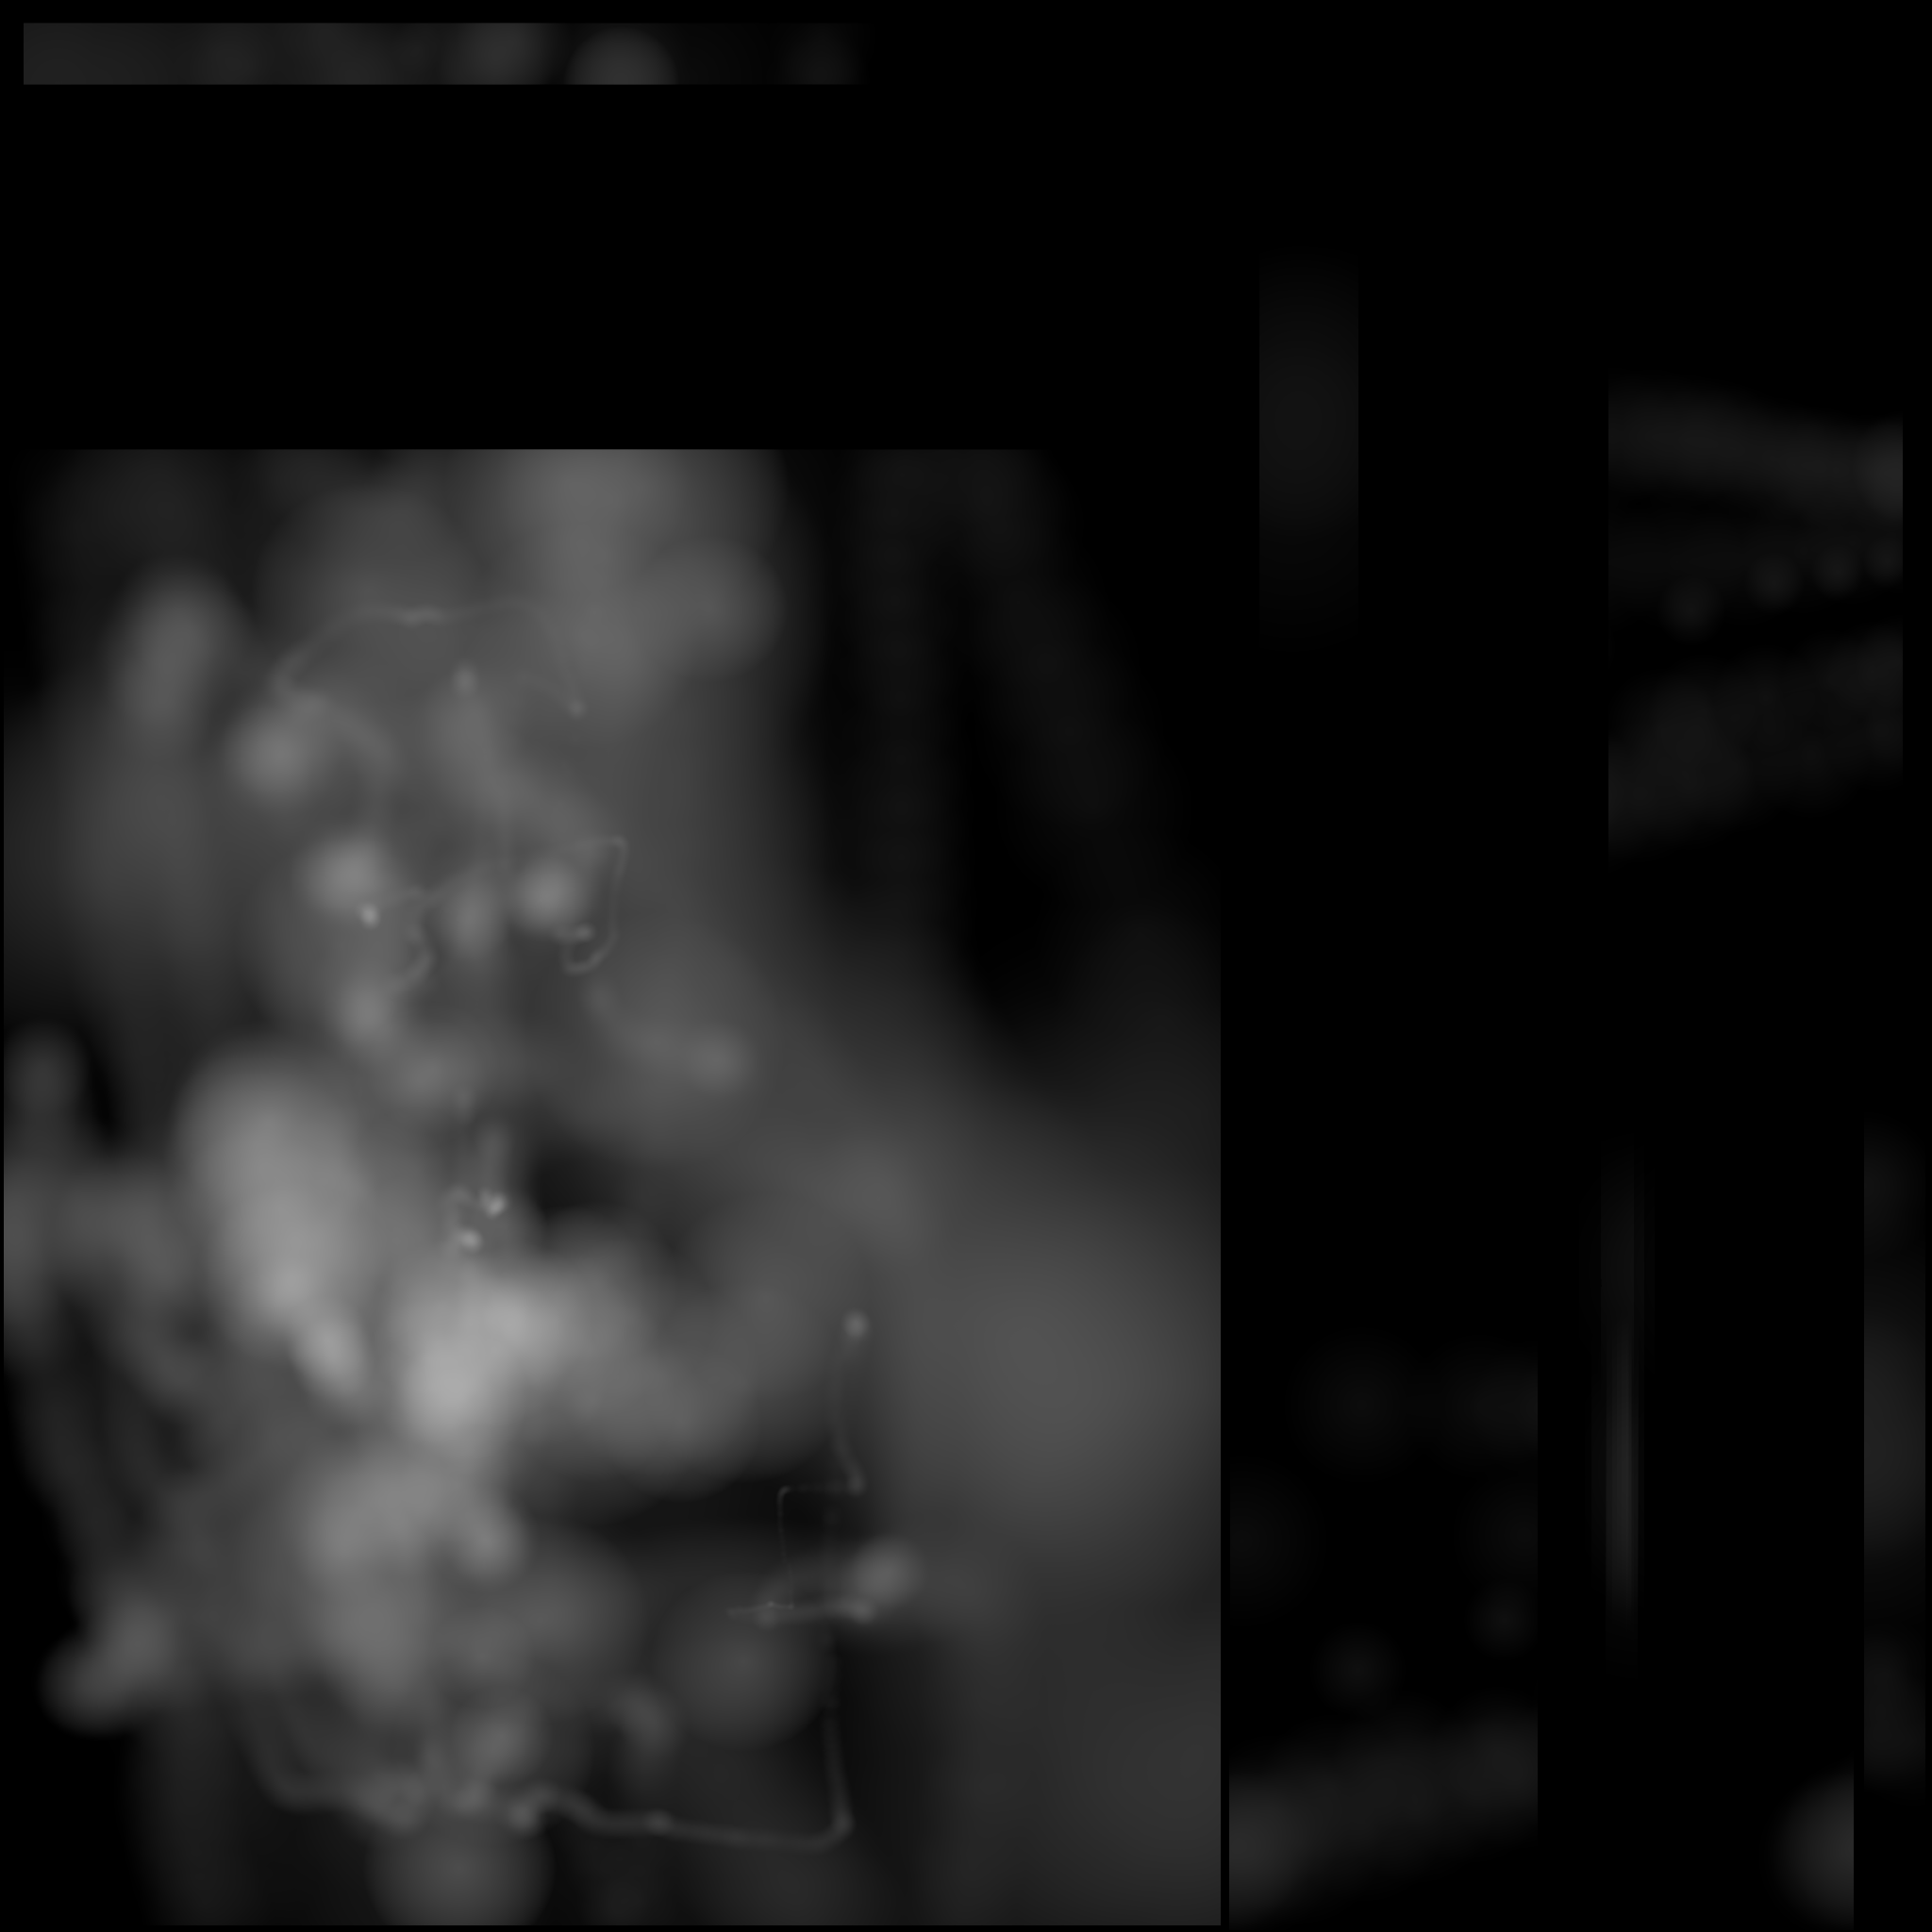
\includegraphics[width=\textwidth]{img/data/Panel14/resultant/Result.png}
        \caption{Result gaze heatmap texture.}
    \end{subfigure}
    \hfill
    \begin{subfigure}[b]{0.325\textwidth}
        \centering
        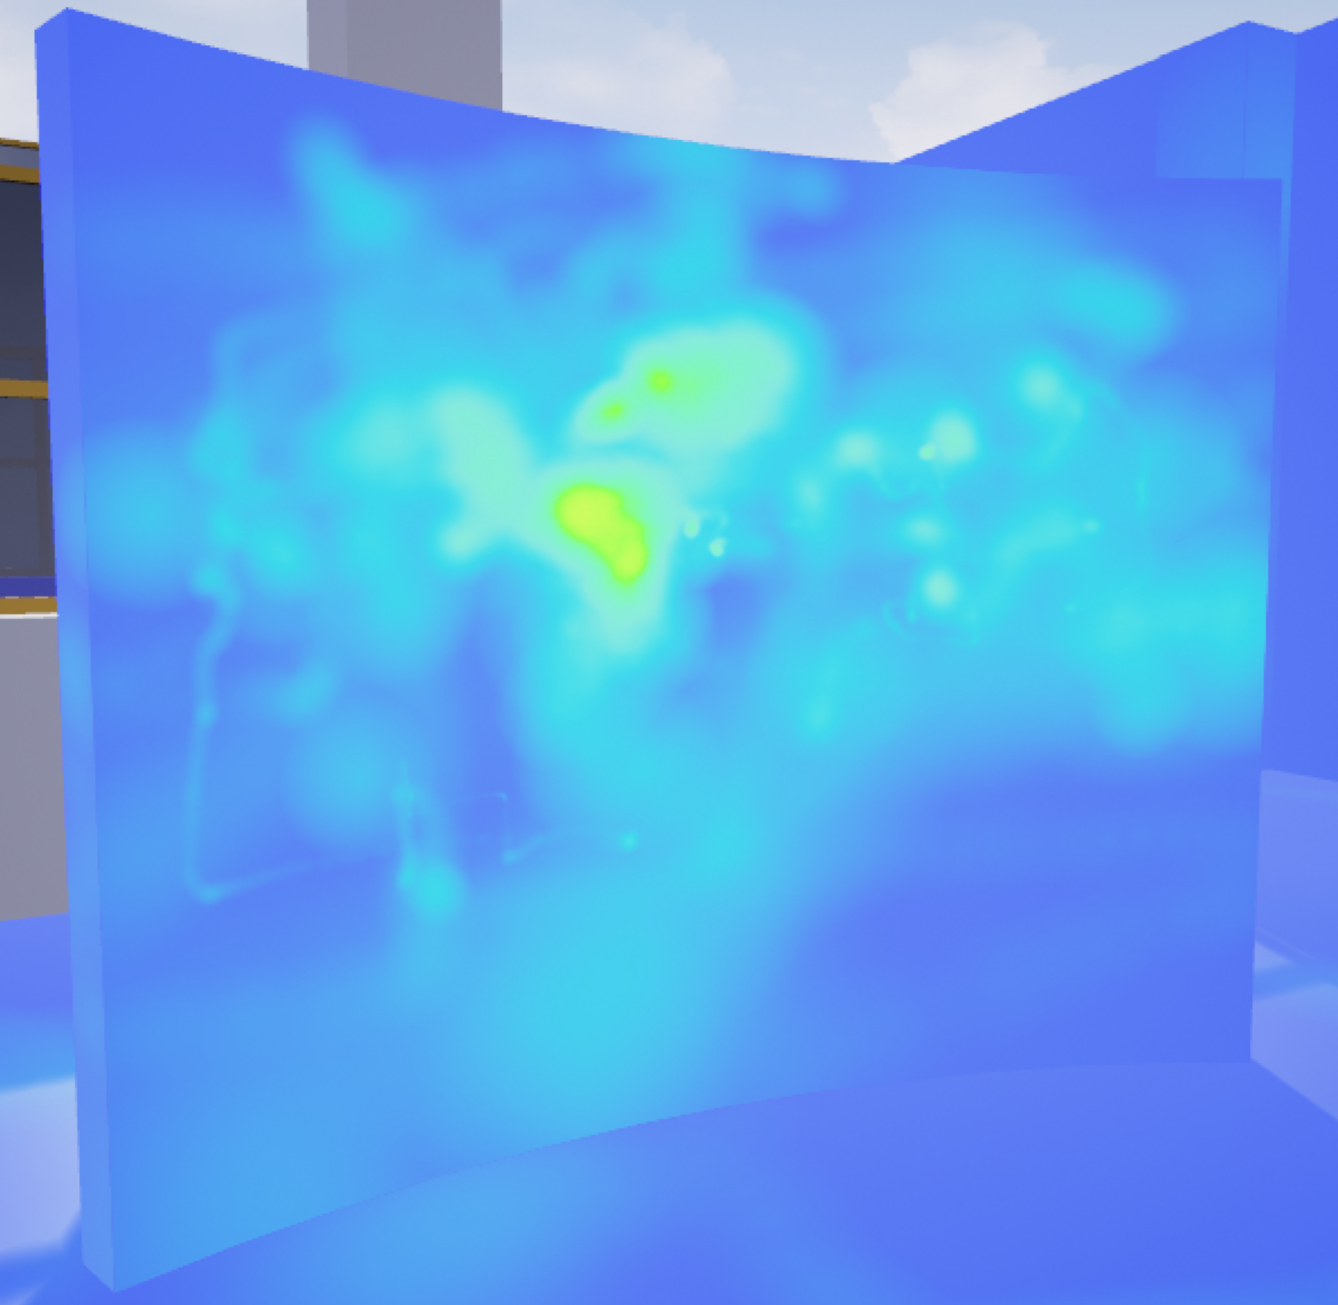
\includegraphics[width=\textwidth]{img/data/Panel14/resultant/heatmap.png}
        \caption{Result gaze heatmap on object.}
    \end{subfigure}
    \hfill
    \begin{subfigure}[b]{0.32\textwidth}
        \centering
        \includegraphics[width=\textwidth]{img/data/Panel14/resultant/original.png}
        \caption{Panel14 original material.}
    \end{subfigure}
    \caption{Resultant heatmap of Panel14.}
    \label{fig:Panel14-resultant-heatmaps.}
\end{figure}



\begin{figure}[!ht]\centering
    \begin{subfigure}[b]{0.24\textwidth}
        \centering
        \includegraphics[width=\textwidth]{img/data/Panel17/single/1.png}
        \caption{Participant 1.}
    \end{subfigure}
    \hfill
    \begin{subfigure}[b]{0.24\textwidth}
        \centering
        \includegraphics[width=\textwidth]{img/data/Panel17/single/2.png}
        \caption{Participant 2.}
    \end{subfigure}
    \hfill
    \begin{subfigure}[b]{0.24\textwidth}
        \centering
        \includegraphics[width=\textwidth]{img/data/Panel17/single/3.png}
        \caption{Participant 3.}
    \end{subfigure}
    \hfill
    \begin{subfigure}[b]{0.24\textwidth}
        \centering
        \includegraphics[width=\textwidth]{img/data/Panel17/single/4.png}
        \caption{Participant 4.}
    \end{subfigure}
    \hfill
    \begin{subfigure}[b]{0.24\textwidth}
        \centering
        \includegraphics[width=\textwidth]{img/data/Panel17/single/5.png}
        \caption{Participant 5.}
    \end{subfigure}
    \hfill    
    \begin{subfigure}[b]{0.24\textwidth}
        \centering
        \includegraphics[width=\textwidth]{img/data/Panel17/single/6.png}
        \caption{Participant 6.}
    \end{subfigure}
    \hfill    
    \begin{subfigure}[b]{0.24\textwidth}
        \centering
        \includegraphics[width=\textwidth]{img/data/Panel17/single/7.png}
        \caption{Participant 7.}
    \end{subfigure}
    \hfill    
    \begin{subfigure}[b]{0.24\textwidth}
        \centering
        \includegraphics[width=\textwidth]{img/data/Panel17/single/8.png}
        \caption{Participant 8.}
    \end{subfigure}
    \hfill    
    \begin{subfigure}[b]{0.24\textwidth}
        \centering
        \includegraphics[width=\textwidth]{img/data/Panel17/single/9.png}
        \caption{Participant 9.}
    \end{subfigure}
    \hfill    
    \begin{subfigure}[b]{0.24\textwidth}
        \centering
        \includegraphics[width=\textwidth]{img/data/Panel17/single/10.png}
        \caption{Participant 10.}
    \end{subfigure}
    \hfill    
    \begin{subfigure}[b]{0.24\textwidth}
        \centering
        \includegraphics[width=\textwidth]{img/data/Panel17/single/11.png}
        \caption{Participant 11.}
    \end{subfigure}
    \hfill    
    \begin{subfigure}[b]{0.24\textwidth}
        \centering
        \includegraphics[width=\textwidth]{img/data/Panel17/single/12.png}
        \caption{Participant 12.}
    \end{subfigure}
    \caption{Heatmap texture variants of Panel17 object.}
    \label{fig:Panel17-object-heatmaps.}
\end{figure}


\begin{figure}[!ht]\centering
    \begin{subfigure}[b]{0.31\textwidth}
        \centering
        \includegraphics[width=\textwidth]{img/data/Panel17/resultant/Result.png}
        \caption{Result gaze heatmap texture.}
    \end{subfigure}
    \hfill
    \begin{subfigure}[b]{0.335\textwidth}
        \centering
        \includegraphics[width=\textwidth]{img/data/Panel17/resultant/heatmap.png}
        \caption{Result gaze heatmap on object.}
    \end{subfigure}
    \hfill
    \begin{subfigure}[b]{0.33\textwidth}
        \centering
        \includegraphics[width=\textwidth]{img/data/Panel17/resultant/original.png}
        \caption{Panel17 original material.}
    \end{subfigure}
    \caption{Resultant heatmap of Panel17.}
    \label{fig:Panel17-resultant-heatmaps.}
\end{figure}

\begin{figure}[!ht]\centering
    \begin{subfigure}[b]{0.24\textwidth}
        \centering
        \includegraphics[width=\textwidth]{img/data/Panel2/single/1.png}
        \caption{Participant 1.}
    \end{subfigure}
    \hfill
    \begin{subfigure}[b]{0.24\textwidth}
        \centering
        \includegraphics[width=\textwidth]{img/data/Panel2/single/2.png}
        \caption{Participant 2.}
    \end{subfigure}
    \hfill
    \begin{subfigure}[b]{0.24\textwidth}
        \centering
        \includegraphics[width=\textwidth]{img/data/Panel2/single/3.png}
        \caption{Participant 3.}
    \end{subfigure}
    \hfill
    \begin{subfigure}[b]{0.24\textwidth}
        \centering
        \includegraphics[width=\textwidth]{img/data/Panel2/single/4.png}
        \caption{Participant 4.}
    \end{subfigure}
    \hfill
    \begin{subfigure}[b]{0.24\textwidth}
        \centering
        \includegraphics[width=\textwidth]{img/data/Panel2/single/5.png}
        \caption{Participant 5.}
    \end{subfigure}
    \hfill    
    \begin{subfigure}[b]{0.24\textwidth}
        \centering
        \includegraphics[width=\textwidth]{img/data/Panel2/single/6.png}
        \caption{Participant 6.}
    \end{subfigure}
    \hfill    
    \begin{subfigure}[b]{0.24\textwidth}
        \centering
        \includegraphics[width=\textwidth]{img/data/Panel2/single/7.png}
        \caption{Participant 7.}
    \end{subfigure}
    \hfill    
    \begin{subfigure}[b]{0.24\textwidth}
        \centering
        \includegraphics[width=\textwidth]{img/data/Panel2/single/8.png}
        \caption{Participant 8.}
    \end{subfigure}
    \hfill    
    \begin{subfigure}[b]{0.24\textwidth}
        \centering
        \includegraphics[width=\textwidth]{img/data/Panel2/single/9.png}
        \caption{Participant 9.}
    \end{subfigure}
    \hfill    
    \begin{subfigure}[b]{0.24\textwidth}
        \centering
        \includegraphics[width=\textwidth]{img/data/Panel2/single/10.png}
        \caption{Participant 10.}
    \end{subfigure}
    \hfill    
    \begin{subfigure}[b]{0.24\textwidth}
        \centering
        \includegraphics[width=\textwidth]{img/data/Panel2/single/11.png}
        \caption{Participant 11.}
    \end{subfigure}
    \hfill    
    \begin{subfigure}[b]{0.24\textwidth}
        \centering
        \includegraphics[width=\textwidth]{img/data/Panel2/single/12.png}
        \caption{Participant 12.}
    \end{subfigure}
    \caption{Heatmap texture variants of Panel2 object.}
    \label{fig:Panel2-object-heatmaps.}
\end{figure}


\begin{figure}[!ht]\centering
    \begin{subfigure}[b]{0.32\textwidth}
        \centering
        \includegraphics[width=\textwidth]{img/data/Panel2/resultant/Result.png}
        \caption{Result gaze heatmap texture.}
    \end{subfigure}
    \hfill
    \begin{subfigure}[b]{0.32\textwidth}
        \centering
        \includegraphics[width=\textwidth]{img/data/Panel2/resultant/heatmap.png}
        \caption{Result gaze heatmap on object.}
    \end{subfigure}
    \hfill
    \begin{subfigure}[b]{0.305\textwidth}
        \centering
        \includegraphics[width=\textwidth]{img/data/Panel2/resultant/original.png}
        \caption{Panel2 original material.}
    \end{subfigure}
    \caption{Resultant heatmap of Panel2.}
    \label{fig:Panel2-resultant-heatmaps.}
\end{figure}